\documentclass{PHlab-thesis}
\usepackage{amsmath}
\usepackage{amsfonts} 
\usepackage{graphicx}
\usepackage{algpseudocode}
\usepackage{algorithm}
\usepackage{enumitem}
\usepackage{subcaption}
\usepackage{booktabs}
\addbibresource{thesis.bib}

\newcommand*\Department中文{人工智慧科技碩士學位學程}
\newcommand*\Department英文{Graduate Program of Artificial Intelligence}

\newcommand*\ThesisTitle中文{加速基因分型---解決MaskedPanGenie效能上的瓶頸}
\newcommand*\ThesisTitle英文{Accelerating Genotyping---Resolving the computational bottleneck of MaskedPanGenie}
%\newcommand*\ThesisNote中文{示例:其實徐翡曼是東京大學畢業的博士}% For real thesis omit, or use {初稿} etc.
%\newcommand*\ThesisNote英文{Just an example.  Fei-Man actually graduated from Tokyo Univ.}% For real thesis omit, or use {draft} etc.

\newcommand*\Student中文{鄭益宗}
\newcommand*\Student英文{Yi-Tsung Cheng}

\newcommand*\Advisor中文{賀保羅}
\newcommand*\Advisor英文{Paul Horton}

%% 果有共同指導老師可以用:
%% \newcommand*\CoAdvisorA中文{}
%% \newcommand*\CoAdvisorA英文{}
%% \newcommand*\CoAdvisorB中文{}
%% \newcommand*\CoAdvisorB英文{}

\newcommand*\YearMonth英文{July, 2023}
\newcommand*\YearMonth中文{112年7月}

\hyphenpenalty=1024

\pagestyle{fancy}
\hyphenation{f-asta}

\begin{document}


% \newcommand*\Keywords英文{genotyping, palindrome spaced seeds, k-mers, alignment free}
% \newcommand*\Abstract英文{Spaced seeds have demonstrated significant improvements in sensitivity for various applications, such as homology search, metagenomic classification, and phylogenetic reconstruction. However, their application in k-mer-based genotyping methods has not been extensively studied. Hartmut Häntze, explored the use of palindrome spaced seeds in PanGenie~\cite{elber2022PanGenie}, namely MaskedPanGenie~\cite{haimo2023MaskedPanGenie}. The results showed that MaskedPanGenie, utilizing palindrome spaced seeds, achieved notable enhancements in genotyping result for both low coverage (5x) and high coverage (30x) scenarios, particularly in capturing indel genotypes. The observed increase in wGC reached up to 6.5\% under high coverage (30x).
% However, it is worth noting that the computational time required for genotyping with MaskedPanGenie was significantly higher, exceeding 3x compared to PanGenie. This contradicts the nature of alignment-free, k-mer-based genotyping methods. In this study, we optimized the MaskedPanGenie pipeline, resulting in approximately 2x faster execution time compared to the original MaskedPanGenie version. Additionally, we investigated the impact of different palindrome spaced seeds for different scenarios on the genotyping results, providing valuable insights for future research on generating optimal palindrome spaced seeds.
% }
\newcommand*\Keywords英文{genotyping, palindrome spaced seeds, k-mer counting, sensitivity}
\newcommand*\Abstract英文{
%Background
Pangenomic approaches are increasingly important for genotyping, inspiring the development of tools such as PanGenie~\cite{elber2022PanGenie}. Recently Häntze \& Horton published MaskedPanGenie~\cite{haimo2023MaskedPanGenie}, which extends the PanGenie approach to support using spaced seeds.  Their results showed enhancements in genotyping performance for both low (5x) and high (30x) read coverage, particularly in capturing indel genotypes.  Promisingly, the observed increase in whole genome concordance reached up to 6.5\% under high coverage (30x).  However their study also had its limitations.  In particular their implementation of MaskedPanGenie is much slower than PanGenie and they tried only a small number of seeds and did not provide a systematic method to generate seeds optimized to the genotyping task.  The work in this report addresses those limitations.

%Method
First, for the speed-up aspect, we propose MaskedJellyfish to enable spaced seed k-mer counting in the MaskedPanGenie pipeline. By incorporating the MaskedJellyfish library for spaced k-mer counting, we eliminate the need for additional preprocessing time in spaced k-mer counting and simplify the MaskedPanGenie pipeline.

Secondly, for seed generation, we propose PalindromeSpEED to generate better palindrome spaced seeds by iteratively optimizing a random seed through flipping and evaluating sensitivity.

%Result
We have two main results.  The first is a very significant (\textasciitilde2X-3X) speed-up over the original MaskedPanGenie workflow.  The second is the development of a method for optimizing spaced seeds for this task and showing that it leads to a modest improvement in performance.
}



% \newcommand*\Keywords中文{基因分析、回文空格種子、k-mers、alignment free}
% \newcommand*\Abstract中文{
% 空格種子(spaced seeds)在各種應用中展示出顯著的靈敏度改善,例如同源性搜索、宏基因組分類和系統發育重建。然而,在基於k-mer的基因分型方法中,對於空格種子的應用尚未得到廣泛研究。因此,作者Hartmut Häntze在PanGenie~\cite{elber2022PanGenie}中增加空格種子的應用並命名為MaskedPanGenie~\cite{haimo2023MaskedPanGenie}。結果顯示,MaskedPanGenie利用空格種子在低覆蓋率(5倍)和高覆蓋率(30倍)情境下均顯著提升了基因分型的結果,特別是在捕捉插入/刪除(indel)方面的表現,在高覆蓋率(30倍)下觀察到的wGC增加可達到6.5\%。
% 然而,值得注意的是,相對於PanGenie,使用MaskedPanGenie進行基因分型所需的計算時間明顯增加至少3倍以上。這與基於k-mer的無比對、基因分型方法的本質上是背道而馳的。在本研究中,我們優化了MaskedPanGenie流程的時間效率,使其執行時間相對於原始版本加快了約2倍。此外,我們還研究了不同狀況間的空格種子對基因分型結果的影響,為後續最佳回文空格種子的研究提供了有價值的見解。
% }
\newcommand*\Keywords中文{基因分型、回文間隔種子、k-mer 計數、敏感度}
\newcommand*\Abstract中文{
全基因組學方法在基因分型中變得越來越重要,啟發了一些工具的開發,如PanGenie~\cite{elber2022PanGenie}。最近Häntze和Horton發表了MaskedPanGenie~\cite{haimo2023MaskedPanGenie},它擴展了PanGenie方法以支援使用間隔種子(spaced seeds)。他們的結果顯示,在低(5倍)和高(30倍)讀取覆蓋率下,特別是捕獲插入/缺失(genotype)方面,基因分型性能有所提升。令人鼓舞的是,在高覆蓋率(30倍)下觀察到的全基因組一致性提高了最多6.5\%。然而,他們的研究也存在一些限制。特別是,他們的MaskedPanGenie執行時間相對於PanGenie慢得多,另外他們只嘗試了少數種子,並沒有提供一種系統方法來生成針對基因分型任務進行優化的種子。本研究解決了這些限制。

首先,在加速方面,我們提出了MaskedJellyfish,用於在MaskedPanGenie流程中實現間隔種子k-mer計數。通過整合MaskedJellyfish庫進行間隔k-mer計數,我們消除了間隔k-mer計數中額外的預處理時間,同時簡化了MaskedPanGenie流程。
其次,在種子生成方面,我們提出了PalindromeSpEED,為了能生成更好的回文間隔種子,通過不斷優化隨機種子和敏感性評估。

我們有兩個主要的結果。第一個結果是相對於原始的MaskedPanGenie工作流程,實現了非常顯著的(約2倍-3倍)加速。第二個結果是開發了一種針對這項任務進行優化的空隔種子方法,並展示了在性能上的適度改進。
}

\newcommand*\Acknowledgements{%

}

\newcommand*\SelectFontsize[2]{\fontsize{#1}{#1}\selectfont\mdseries#2\par}
\newcommand*\SelectFontsizeBF[2]{\fontsize{#1}{#1}\selectfont\bfseries#2\par}
\newcommand*\SignatureRule[1][6]{\rule{#1cm}{0.3mm}}
\newcommand*\AddToContents[1]{\newpage\phantomsection\addcontentsline{toc}{chapter}{#1}}

\doublespace
\pagenumbering{gobble}
\renewcommand{\thefootnote}{\fnsymbol{footnote}}


\begin{center}
\vspace{2cm}
\SelectFontsizeBF{23}{%
\University中文\Department中文\\
\學位 論文}

\vfill
\SelectFontsizeBF{24}{\ThesisTitle中文}
\ifdefined\ThesisNote中文
\SelectFontsize{22}{\textit{\ThesisNote中文}}
\fi

\vspace{5mm}
\SelectFontsizeBF{22}{\ThesisTitle英文}
\ifdefined\ThesisNote英文
\SelectFontsize{20}{\textit{\ThesisNote英文}}
\fi

\vfill

\begin{minipage}{\linewidth}
{\setlength\tabcolsep{0pt}
%
\begin{tabular}{ Wr{5em} Wl{5em} Wr{5em} wl{7em} }
研究生:   & ~~\Student中文  &      Student: & ~~\Student英文\\
指導老師: & ~~\Advisor中文  &      Advisor: & ~~\Advisor英文\\
\ifdefined\CoAdvisorA中文
共同指導: & ~~\CoAdvisorA中文 &   Co-Advisor: & ~~\CoAdvisorA英文\\
\fi
\ifdefined\CoAdvisorB中文
         & ~~\CoAdvisorB中文 &   Co-Advisor: & ~~\CoAdvisorB英文\\
\fi
\end{tabular}
}
\end{minipage}

\vfill
\SelectFontsize{18}{%
National Cheng Kung University,\\
Tainan, Taiwan, R.O.C.\\
Thesis for \ifdef\PhD{Doctor of Philosophy}{Master of Science} Degree\\
\YearMonth英文}

\vfill
\SelectFontsize{20}{中華民國\YearMonth中文}
\end{center}



\ifdefined\optCommittee
\newpage
\begin{center}
\vspace{1cm}
\SelectFontsizeBF{24}{%
\University中文\Department中文\\
\學位 論文}
\vfill
\SelectFontsizeBF{20}{\ThesisTitle中文}
\end{center}

\vfill
\SelectFontsize{20}{%
\noindent 研究生:\Student中文\\
本論文業經審查及口試合格特此證明}


\begin{center}
\SelectFontsize{18pt}{論文考試委員}
\vfill
\SignatureRule \hspace*{1cm} \SignatureRule
\vfill

\SignatureRule \hspace*{1cm} \SignatureRule
\vfill

指導教授:\SignatureRule[8]
\vfill
  所長:\SignatureRule[8]

\vfill
\SelectFontsize{18}{中華民國 \hspace{2em} 年 \hspace{2em} 月 \hspace{2em} 日}
\end{center}


\newpage
\begin{center}
\vspace{1cm}
\SelectFontsize{18}{\University英文, \Department英文}
\SelectFontsize{19}{\ifdef\PhD{Ph.D.}{Master's} Degree Thesis}

\vfill
\SelectFontsizeBF{20}{\ThesisTitle英文}
\end{center}

\vfill
\SelectFontsize{18}{Student: \Student英文}

\SelectFontsize{18}{%
A thesis submitted to the graduate division in partial fulfillment of the requirement for the degree of
\ifdef\PhD{Doctor of \mbox{Philosophy}}{Master of Science}.
}

\vfill
\begin{center}
\SelectFontsize{18}{Approved by}

\vfill
\SignatureRule \hspace*{1cm} \SignatureRule

\vfill
\SignatureRule \hspace*{1cm} \SignatureRule

\vfill
Advisor: \SignatureRule[8]

\vfill
Chairman: \SignatureRule[8]

\vfill
\SelectFontsize{18}{\YearMonth英文}
\vspace*{20pt}
\end{center}
\fi% optCommittee


\AddToContents{中文摘要}
\setcounter{page}{1}
\pagenumbering{roman}


\begin{center}
\SelectFontsizeBF{24}{\ThesisTitle中文}

\vspace{4mm}
\SelectFontsize{18}{\Student中文\footnote[1]{學生} ~ \Advisor中文\footnote[2]{指導教授}}

\vspace{5mm}
\SelectFontsize{20}{國立成功大學\Department中文}

\vspace{12mm}
\makebox[2.7cm][c]{\SelectFontsizeBF{22}{摘要}}
\end{center}

\vspace{4mm}
\SelectFontsize{16}{\Abstract中文}

\vspace{4mm}
\begin{flushleft}
\SelectFontsize{16}{\textbf{關鍵詞:} \Keywords中文}
\end{flushleft}



\AddToContents{Abstract}
\begin{center}
\SelectFontsizeBF{22}{\ThesisTitle英文}

\vspace{4mm}
\SelectFontsize{18}{\Student英文\footnote[1]{Student} ~ \Advisor英文\footnote[2]{Advisor}}

\vspace{4mm}
\SelectFontsize{16}{\Department英文, National Cheng Kung University}

\vspace{12mm}
\SelectFontsizeBF{20}{Abstract}
\end{center}

\vspace{4mm}
\SelectFontsize{14}{\Abstract英文}

\vspace{4mm}
\begin{flushleft}
\SelectFontsize{16}{\textbf{Keywords:} \Keywords英文}
\end{flushleft}



\AddToContents{誌謝}
\begin{center}\SelectFontsizeBF{24}{誌謝}\end{center}

\vspace{4mm}
\Acknowledgements



\renewcommand{\contentsname}{CONTENTS}
\AddToContents{Contents}
\tableofcontents


\AddToContents{List of Tables}
\listoftables


\AddToContents{List of Figures}
\listoffigures
% 封面頁, 口委中英文簽名單, 誌謝, 中英文摘要, 論文目錄, 圖表目錄


%────────────────────  List of Symbols  ────────────────────
\renewcommand\nomgroup[1]{%
  \item[\bfseries
  \ifstrequal{#1}{A}{General}{%
  \ifstrequal{#1}{B}{Metrics}{%
  \ifstrequal{#1}{C}{Variants}{%
  \ifstrequal{#1}{Z}{Gene/Protein Names}%
  }}}]}

% \nomenclature[A]{$\lg$}{Logarithm base 2}
% \nomenclature[A]{KL\ Divergence}{Kullback-Liebler Divergence}
% \nomenclature[Z]{Myc}{MYC proto-oncogene}
% \nomenclature[Z]{USF-1}{Upstream stimulatory factor 1}
\nomenclature[A]{HMM}{Hidden Markov Model}
\nomenclature[B]{wGC}{weighted genotype concordance}
\nomenclature[C]{bp}{base pair}
\nomenclature[C]{indel}{Insertion / Deletion}
\nomenclature[C]{SNV}{Single nucleotide variation}
\nomenclature[C]{SV}{Structural variation}

\printnomenclature[5cm]

\newpage
\setcounter{page}{1}
\pagenumbering{arabic}


\chapter{Introduction}
Spaced seeds have been shown to improve the performance of many sequence analysis and alignment algorithms in bioinformatics. Traditional methods rely on contiguous subsequences, known as contiguous seeds, for similarity search and alignment. A prominent example is Blast~\cite{ALTSCHUL1990Blast}, which adopts the "hit and extend" approach. In this method, a hit is defined as an exact match of 11 consecutive nucleotides between two sequences, and these matches serve as potential candidates for extension and local alignment. However, it is evident that not all local alignments exhibit an identical stretch of length 11. This limitation highlights the constrained nature of contiguous seeds in handling sequence variations.

Spaced seeds address this limitation by allowing for "don't care" positions within the seed. These positions can match any nucleotide or tolerate variations, thus providing flexibility in accommodating sequence variations. By incorporating spaced seeds into alignment algorithms, researchers can improve sensitivity and specificity, especially in cases where the sequences being compared contain variations or have different lengths.

The concept of spaced seeds was initially introduced by Ma et al. and was subsequently implemented in the PatternHunter~\cite{MaB2002PatternHunter} software. Spaced seeds have demonstrated their effectiveness in enhancing sensitivity for homology search and was sucessfully applied in various bioinformatics tasks, including metagenome sequence clustering, protein classification, read mapping, phylogeny reconstruction. They have demonstrated their effectiveness in improving alignment accuracy, reducing computational time, and enabling the analysis of large-scale genomic datasets.

Several software tools have been developed to generate approximate optimal spaced seeds, including SpEED~\cite{Lucian2011SpEED}, RasBhari~\cite{Hahn2016Rasbhari}, and Iedera~\cite{Kucherov2006Sensitivity}. These tools aim to optimize seed parameters, such as seed length, seed weight, and seed spacing, to maximize the sensitivity and specificity of seed-based algorithms. They employ different methods and algorithms to achieve seed optimization, resulting in improved performance and results for various genomic analysis tasks. Utilizing these tools can assist researchers in selecting the most suitable seed parameters for specific applications and datasets, thereby enhancing the accuracy and efficiency of alignment-free, k-mer-based algorithms in sequence analysis.

MaskedPanGenie incorporates approximate optimal spaced seeds to enhance the alignment-free k-mer-based genotyper, PanGenie.This integration of spaced seeds improves the recall, F-score, and weighted genotype concordance (wGC) of PanGenie when genotyping SNPs, indels, and structural variations (SV) in reads with low (5x) and high (30x) coverage. Notably, significant improvements are observed in the genotyping accuracy of indels, with wGC increasing by up to 6.5\% at 30-fold coverage. These results highlight the efficacy of utilizing spaced seeds over simply increasing the length of contiguous k-mers in PanGenie, ultimately enhancing its performance in variant genotyping across different coverage scenarios.

However, MaskedPanGenie suffers from certain concerns.
\begin{enumerate}[label=(\roman*)]
    \item High runtime: Compared to the original PanGenie's contiguous k-mer approach, MaskedPanGenie's runtime becomes significantly longer. This discrepancy worsens with parallelization on multicore systems. This prolonged runtime poses inconveniences to users and raises questions about the acceptability of the time cost, especially considering PanGenie's primary purpose of accelerating genotyping with an alignment-free k-mer-based method compared to reference mapping approaches.
    \item Selection of spaced seeds:The choice of spaced seeds plays a crucial role in genotyping result, as evidenced by various studies. Due to software limitations, the author employs SpEED~\cite{Lucian2011SpEED} to generate shorter approximate optimal spaced seeds and then extends them with their mirrored version on the right side to ensure palindromicity. While this approach yields palindrome spaced seeds, it does not guarantee approximately optimal palindrome spaced seeds. Hence, our research also investigates which spaced seed patterns yield better genotyping results. Additionally, we validate the impact of spaced seeds on the genotyping outcomes.
\end{enumerate}
Based on the aforementioned concerns, we propose two solutions and provide discussions.
\begin{enumerate}[label=(\roman*)]
    \item Addressing the issue of high runtime: We will optimize the MaskedPanGenie pipeline to significantly reduce the additional data processing and computational time, thereby mitigating the impact of time costs. This optimization aims to alleviate the inconvenience caused to users and ensure a more efficient genotyping process.
    \item Enhancing the selection of spaced seeds: Building upon the SpEED algorithm, we will develop an modified approach capable of generating approximate optimal palindrome spaced seeds. This revised method ensures a more reasonable selection process for spaced seeds, in contrast to the current practice of obtaining palindrome spaced seeds. Additionally, in the results chapter, we will examine the genotyping outcomes under different scenarios using spaced seeds, including those derived from the author's original approach.
\end{enumerate}



\chapter{Background \& Related Work}
In this chapter, we provide an overview of the literature that forms the basis of this thesis. The first section provides an introduction to spaced seeds. The second section focuses on understanding the relevant tools, as this research builds upon the MaskedPanGenie pipeline. It aims to enhance our understanding of the tools' usage and later modifications within the MaskedPanGenie pipeline. The third section begins by introducing the application of PanGenie and then delves into a detailed explanation and integration of the MaskedPanGenie pipeline.
\section{Spaced Seeds}
\subsection{Notation}
A spaced seed $S$ is a string consisting of 1s and 0s, representing matching positions and non-matching positions or wildcards, respectively~\cite{Petrucci2020ISSH}. For instance, a spaced seed can be represented as 1011110 , where 1s requires a match in that position and 0s allows for "don't care". The weight of a spaced seed, denoted as $W$, is the count of 1s in the seed, while the length or span is the sum of the number of 0s and 1s.

In notation introduced in~\cite{Keich2004Spacedseeds}, a spaced seed can be denoted by its shape, represented as $Q$. The weight $W$ of the seed is indicated by $\left | Q \right |$, and the length or span $s(Q)$ = max($Q$)+1. For example, if we have $Q=\{0, 2, 4, 6\}$, it corresponds to the spaced seed $S=1010101$, span $s(Q)=7$ and weight $\left | Q \right | = 4$ .
Given a string $x$, the positioned spaced seed $x[i+Q]$ identifies a string of length $\left | Q \right |$, where $0\leq i\leq n-s(Q)$. The positioned spaced seed $x[i+Q]$, also known as a Q-gram, is defined as the string $\{x[i+Q] = {x_{i+k},k\in Q}\}$.

Example2.1: Consider the string $x$ = ACTCAGTCG, with the spaced seed = 1011101. We will know $Q$ = \{0, 2, 3, 4, 6\}, with weight $\left| Q \right | = 5$ and length(span) s(Q) = 7. 
\begin{center}   
\begin{tabular}{ccccccccccc}
x& & A & C & T & C & A & G & T & C & G\\
Q& & 1 & 0 & 1 & 1 & 1 & 0 & 1 & &\\
x[0+Q] & & A & & T & C & A & & T & &\\
\end{tabular}
\end{center} 
We can also get x[1 + Q] = CCAGC and x[2 + Q] = TAGTG. By shifting the position by $i$, we obtain the corresponding string results, where $0\leq i\leq 2$ .

    
\subsection{Palindrome spaced seeds}
MaskedPanGenie utilizes the canonical representation of k-mers, where each k-mer is treated as equivalent to its reverse complement, and the lexicographically smaller version is selected as the representative. However, it is important to note that the canonical form of spaced k-mers may not necessarily be the same as their reverse strand. For example, if the spaced seed is 11001 (length = 5, W = 3), consider the sequence GACTA on the forward strand and, conversely, TAGTC on the reverse strand. The resulting 3-mer for the forward strand is GAA and TAC for the reverse strand. Their canonical forms are CTT and ATG, respectively. This is the reason why we need to use palindrome spaced seeds, as they ensure that the canonical form of both the forward and reverse strands is equal.

In this section, we define palindrome spaced seeds as follows:
Given a spaced seed $S = "s_0, s_1, ..., s_{n-1}"$, where $s_i$ represents the elements of the seed and $n$ is the length of the seed, a spaced seed is considered a palindrome spaced seed if $\forall i \in [0, \lfloor \frac{n}{2} \rfloor]$, $s_i = s_{n-i-1}$. This means that the elements of the spaced seed are symmetric around the center, creating a palindrome structure. For example, consider the spaced seed S = "11011", which is a palindrome spaced seed.
Additionally, it is important to mention that this study will not include spaced seeds with trailing and leading zeros. This is because the presence of leading and trailing zeros in spaced seeds does not impact the composition of the selected k-mers. Therefore, this study focuses only on palindrome spaced seeds in the form of "1s1".

\section{Related tools}
\subsection{Optimal spaced seed - SpEED}
Finding an optimal spaced seed is a challenging task known to be NP-hard. It involves two exponential-time problems:
\begin{enumerate}[label=(\roman*)]
    \item The large number of spaced seed candidates to be considered leads to an exponential search space~\cite{MA2007complexitySpaced}.
    \item Computing the sensitivity of each spaced seed also requires exponential time~\cite{MA2007complexitySpaced}.
\end{enumerate}
In this section, we aim to understand the concept of sensitivity for spaced seeds(ii). However, due to its computational complexity, we seek an alternative metric that can effectively assess the quality of a spaced seed in polynomial time. This metric will allow us to efficiently identify good spaced seeds for our purposes. Furthermore, we will explain how SpEED addresses the issue of selecting the optimal seed length among the numerous spaced seed candidates(i).
\subsubsection{Concept of sensitivity}
The sensitivity of a seed refers to the probability of correctly identifying a similar region of a specific length in a random sequence. In other words, the sensitivity can be used as a measure to evaluate the effetiveness of spaced seeds in detecting similar regions between biological sequences~\cite{haimo2023MaskedPanGenie}~\cite{MaB2002PatternHunter}. Intuitively, sensitivity provides insights into the ability of a seed to accurately detect regions of similarity in sequences.

Although sensitivity can be computed using dynamic programming~\cite{MA2007complexitySpaced} or recurrent relations~\cite{Choi2004recurrent}, these algorithms still have exponential time complexity. This means that using sensitivity as a measure to evaluate the quality of spaced seeds can be time-consuming.

However, Ilie and Ilie~\cite{Ilie2007SpacedSeed} introduced a new evaluation metric called overlap complexity, which has been shown through experimental results to be highly correlated with sensitivity. The computation of overlap complexity can be achieved in polynomial time.
\subsubsection{Overlap complexity}
According to this study, the overlap complexity~\cite{Ilie2007Long} of a seed $s$ is formally defined as follows:
\begin{equation}
    OC(s) = \sum\limits_{i = 1}^{l-1}2^{\sigma[i]}
\end{equation}\\Here, $\sigma[i]$ represents the number of pairs of 1's between $s$ and its shifted version at position $i$. A lower number of overlap care positions indicates better sensitivity for the spaced seed. As the overlap complexity decreases, the sensitivity of the spaced seed increases, and vice versa.

Example2.2:\\
Consider the spaced seed $S$ = 10101. The computation of overlap complexity for this spaced seed is performed as follows:\\  
\begin{tabular}{ccccccccccccc}
  &   &   &   &   &   &   &   &   &   &   & shift i & $\sigma[i]$ \\
1 & 0 & 1 & 0 & 1 & * & * & * & * & * & * &         &            \\
* & 1 & 0 & 1 & 0 & 1 & * & * & * & * & * &   1     &     0      \\
* & * & 1 & 0 & 1 & 0 & 1 & * & * & * & * &   2     &     2       \\
* & * & * & 1 & 0 & 1 & 0 & 1 & * & * & * &   3     &     0        \\
* & * & * & * & 1 & 0 & 1 & 0 & 1 & * & * &   4     &     1        \\
\end{tabular}\\\\\\
We can get OC($S$) = $\sum\limits_{i = 1}^{l = 4}2^{\sigma[i]}$ = 0 + 2 + 0 + 1 = 3. Overlap complexity provides a reliable estimation of sensitivity and can be computed efficiently in low polynomial time. 
\subsubsection{SpEED}
The Ilie and Ilie (2007) algorithm relies on user-defined seed lengths, but which seed length is best. In SpEED, the authors have addressed this issue by developing a preprocessing algorithm that computes a range of good seed lengths. This algorithm computes all possible seed lengths between the minimum and maximum values, allowing for greater flexibility in selecting optimal seed lengths. Hartmut Häntze (2023) mentioned that Ilie and Ilie (2011) conducted tests on their algorithm for multiple spaced seeds, with a maximum weight of 18~\cite{haimo2023MaskedPanGenie}. However, MaskedPanGenie is designed for mid-size k-mers with a weight of 31. Therefore, it is unclear that SpEED may not be able to provide approximate optimal spaced seeds for this weight. As a result,  Hartmut Häntze used a more suitable approach to generate spaced seeds with a weight of 31 for the execution MaskedPanGenie.
\subsection{K-mer counting - Jellyfish}
The task of k-mer counting is to count the number of substrings of length k in a string $S$ or a set of strings. The traditional approach involves using a dictionary structure with k-mers as keys and their counts as values. However, with the advent of high-throughput sequencing technologies~\cite{Reu2015Sequencing}, such as next-generation sequencing (NGS), which produce a massive amount of short sequences, optimizing time and memory usage becomes crucial.

To address this challenge, various k-mer counting algorithms have been developed to optimize time and space efficiency. According to a comprehensive review~\cite{Man2018benchmark}, the main approaches for k-mer counting include hash tables, sorting, burst tries, and enhanced suffix arrays. Furthermore, these methods can be categorized into two major classes based on memory usage: disk-based or in-memory approaches. Disk-based approaches, also known as external memory or out-of-core approaches, aim to reduce memory consumption.

For counting k-mers in reads and pangenome graphs, the PanGenie tool utilizes Jellyfish. Jellyfish~\cite{Mar2011Jellyfish} employs a lock-free hash table and parallelization techniques to insert k-mers and update their frequencies concurrently. To ensure efficiency and correctness, it utilizes the hardware instruction compare-and-swap (CAS) to guarantee the integrity of frequency updates. The workflow of Jellyfish can be summarized as follows: (i) If a k-mer is not found in the hash table, a reprobing strategy is used to insert the k-mer as a new key with a frequency set to 1. (ii) If the k-mer already exists, its frequency count is incremented by 1. (iii) In case of collisions, a quadratic probing method is employed to resolve them. By utilizing CAS, Jellyfish prevents concurrent threads from simultaneously modifying the frequency value of the same memory location, thereby ensuring accurate results and avoiding data corruption.
\subsection{Metrics for genotyping results - GenotypeConcordance}
In the results chapter, various evaluation metrics are used to assess the impact of spaced seeds on genotyping result. The evaluation metrics include recall, precision, F-score, and genotype concordance.
\begin{center}
    recall = $\frac{TP}{TP + FN}$\hspace{0.5cm}precision = $\frac{TP}{TP + FP}$\hspace{0.5cm}F-score = 2 * $\dfrac{\text{precsion}*\text{recall}}{\text{precision} + \text{recall}}$
\end{center}

Recall, precision, and F-score are used to measure the differences between the predicted haplotypes and the true set of haplotypes. Variants in the predicted callsets can be classified as absent (0|0), heterozygous (1|0), homozygous (1|1), or undefined (*|*). True positive (TP), false positive (FP), and false negative (FN) are defined based on the most stringent model of "Best practices for benchmarking germline small-variant calls in human genomes."~\cite{Peter2019Metrics} TP refers to sides with identical alleles and genotype in both the truth and callset, while homozygous reference alleles are not counted as TPs for precision and recall.

Genotype concordance, which measures the proportion of correctly genotyped variants, is another metric for comparing callsets. However, genotype concordance may be biased when callsets contain variants from multiple samples, as the number of absent variants (0|0) can be higher than the number of variants with true genotypes (0|1 or 1|1). To address this, weighted genotype concordance (wGC) is used, where the number of correctly and erroneously classified variants of genotype x|y are labeled as Tx|y and Fx|y, respectively.
\begin{center}
    conc(0|0) = $\frac{T_{0|0}}{T_{0|0} + F_{0|0}}$\hspace{0.5cm}conc(0|1) = $\frac{T_{0|1}}{T_{0|1} + F_{0|1}}$\hspace{0.5cm} conc(1|1) = $\frac{T_{1|1}}{T_{1|1} + F_{1|1}}$\\
    \vspace{1cm}
    wGC = $\frac{\text{conc(0|0)} + \text{conc(0|1)} + \text{conc(1|1)}}{3}$
\end{center}

In this study, adjusted versions of these metrics are reported, considering only variants present in the given variant file (vcf). Variants that are undefined in the ground-truth set are removed from both sets to ensure consistency in the evaluation.
\section{MaskedPanGenie}
\subsubsection{PanGenie}
\begin{figure}
	\centering
	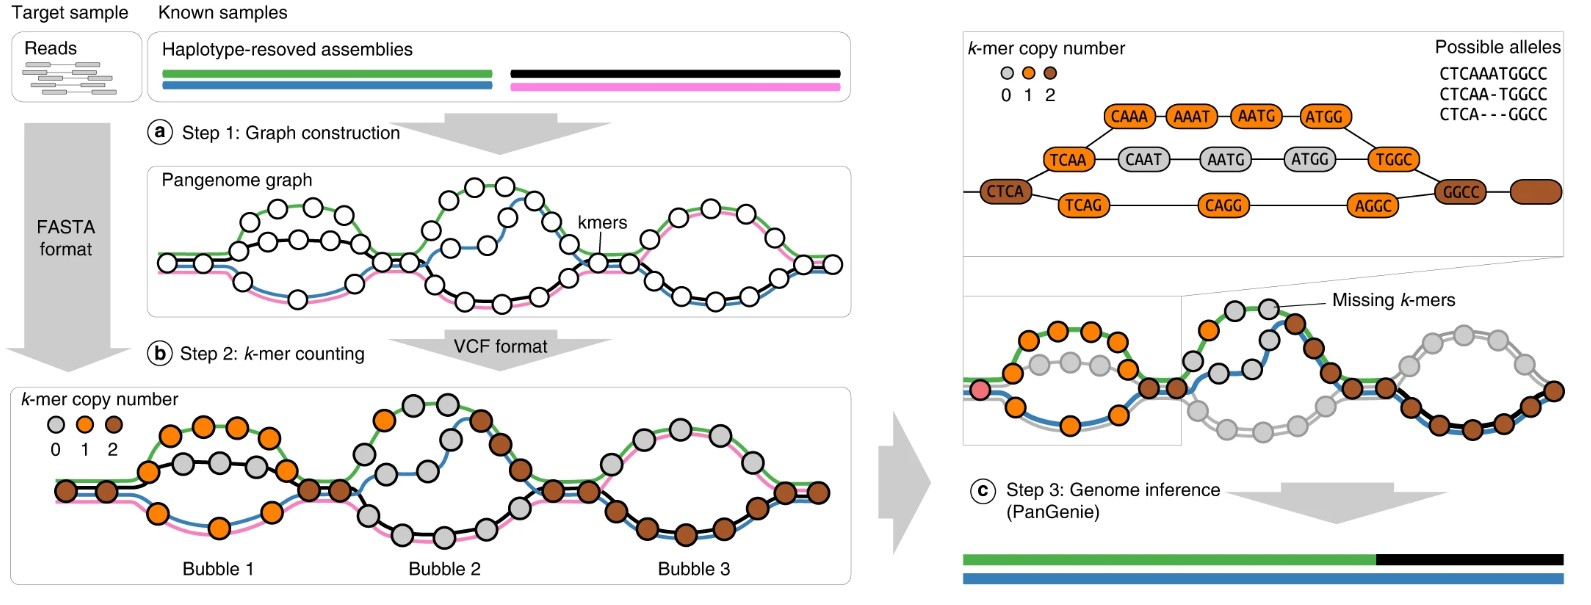
\includegraphics[scale=0.4]{figures/workflow of PanGenie.jpg}
	\caption{Workflow of PanGenie (Figure is taken from~\cite{1}, without changes, and is under a Creative Commons License.(\url{https://creativecommons.org/licenses/by/4.0/}))}
	\label{fig:PanGenie} % \ref{this label}
\end{figure}
PanGenie, a novel algorithm for genotyping genetic variants using a haplotype-resolved pangenome reference and k-mer counts from short-read sequencing data~\cite{elber2022PanGenie}. Traditional genotyping workflows rely on aligning reads to a reference genome, which introduces biases and computational complexity. PanGenie overcomes these limitations by leveraging the pangenome graph, constructed from multiple haplotype-resolved assemblies, to represent variants as bubbles with different allele paths~\cite{elber2022PanGenie}.

To genotype the bubbles, PanGenie compares the expected counts of k-mers unique to each bubble with the actual k-mer counts in the reads (Figure \ref{fig:PanGenie}). The expected counts depend on the number of alleles the k-mer is part of and the mean k-mer coverage. Poisson and geometric distributions are used to model k-mer counts for alleles present in both or only one allele, respectively. Genotypes of neighboring positions are used to calculate the posterior probability of allele combinations, taking advantage of linkage disequilibrium (LD) patterns observed at the population level.

PanGenie utilizes a hidden Markov model (HMM) to leverage LD and make assumptions about the genotypes of poorly covered alleles. The HMM's hidden states represent pairs of haplotype paths in the variant graph, and the observations are the counts of unique k-mers covering each bubble. Transition probabilities in the HMM are calculated based on LD, following the Li-Stephens model~\cite{Li2003linkage}. The likelihoods of haplotype paths, calculated earlier, serve as the emission probabilities for the HMM. The most likely pairs of haplotype paths at each bubble position are determined using the forward-backward algorithm.

Compared to mapping-based algorithms, PanGenie offers significant improvements in speed and genotype concordance for various variant types and coverages. It performs particularly well in repetitive regions and large insertions. However, PanGenie only utilizes contiguous k-mers, despite reports that spaced seeds can enhance many k-mer-based algorithms.

In summary, PanGenie provides a fast and accurate approach for genotyping genetic variants by leveraging haplotype-resolved assemblies and k-mer counts. It surpasses traditional mapping-based methods and enables the inclusion of variants in repetitive regions, expanding the scope of genome-wide association studies.
\subsection{MaskedPanGenie pipeline}
The use of approximate optimal spaced seed improves the genotyping results of MaskedPanGenie. For example, consider a sequence with a variant site. Previous research has shown that variants in the genome exhibit specific patterns of surrounding k-mers. By analyzing the observed patterns, likelihoods for the reference and alternative alleles can be calculated.

However, challenges arise when there is a base mutation near the variant site or sequencing errors in the reads covering the site(see Figure 2.2). These factors make it difficult to accurately identify the variant, thus affecting the final genotyping result.

By employing approximate optimal spaced seed, MaskedPanGenie addresses these challenges more effectively. Approximate optimal spaced seed incorporates care and don't care positions, allowing for flexible matching. The spaced seed model accommodates mutations by allowing for some mismatches in predefined positions. Moreover, from a statistical perspective, the occurrences of spaced seeds at neighboring sequence positions are statistically less dependent than contiguous k-mers~\cite{Girotto2018FSH}.\\
\begin{figure}
	\centering
    \begin{subfigure}[t]{0.48\textwidth}
        \centering
        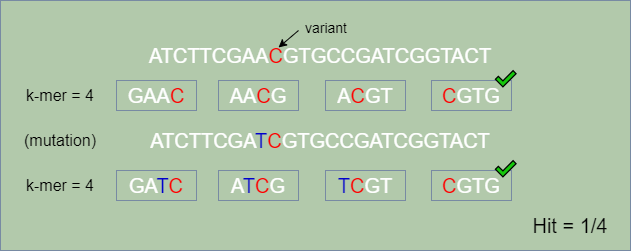
\includegraphics[width=\textwidth]{figures/spaced_seed_mutation.drawio (5).png}
        \label{fig:MaskedPanGenie_fig1}
    \end{subfigure}
    \hfill
    \begin{subfigure}[t]{0.48\textwidth}
        \centering
        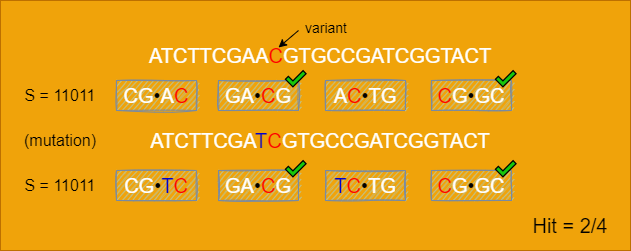
\includegraphics[width=\textwidth]{figures/spaced_seed_mutation.drawio (9).png}
        \label{fig:MaskedPanGenie_fig2}
    \end{subfigure}
    \caption{Spaced seeds are more sensitive}
\end{figure}
Overview the overall process of MaskedPanGenie(see Figure \ref{fig:MaskedPanGenie}):
\begin{figure}
	\centering
	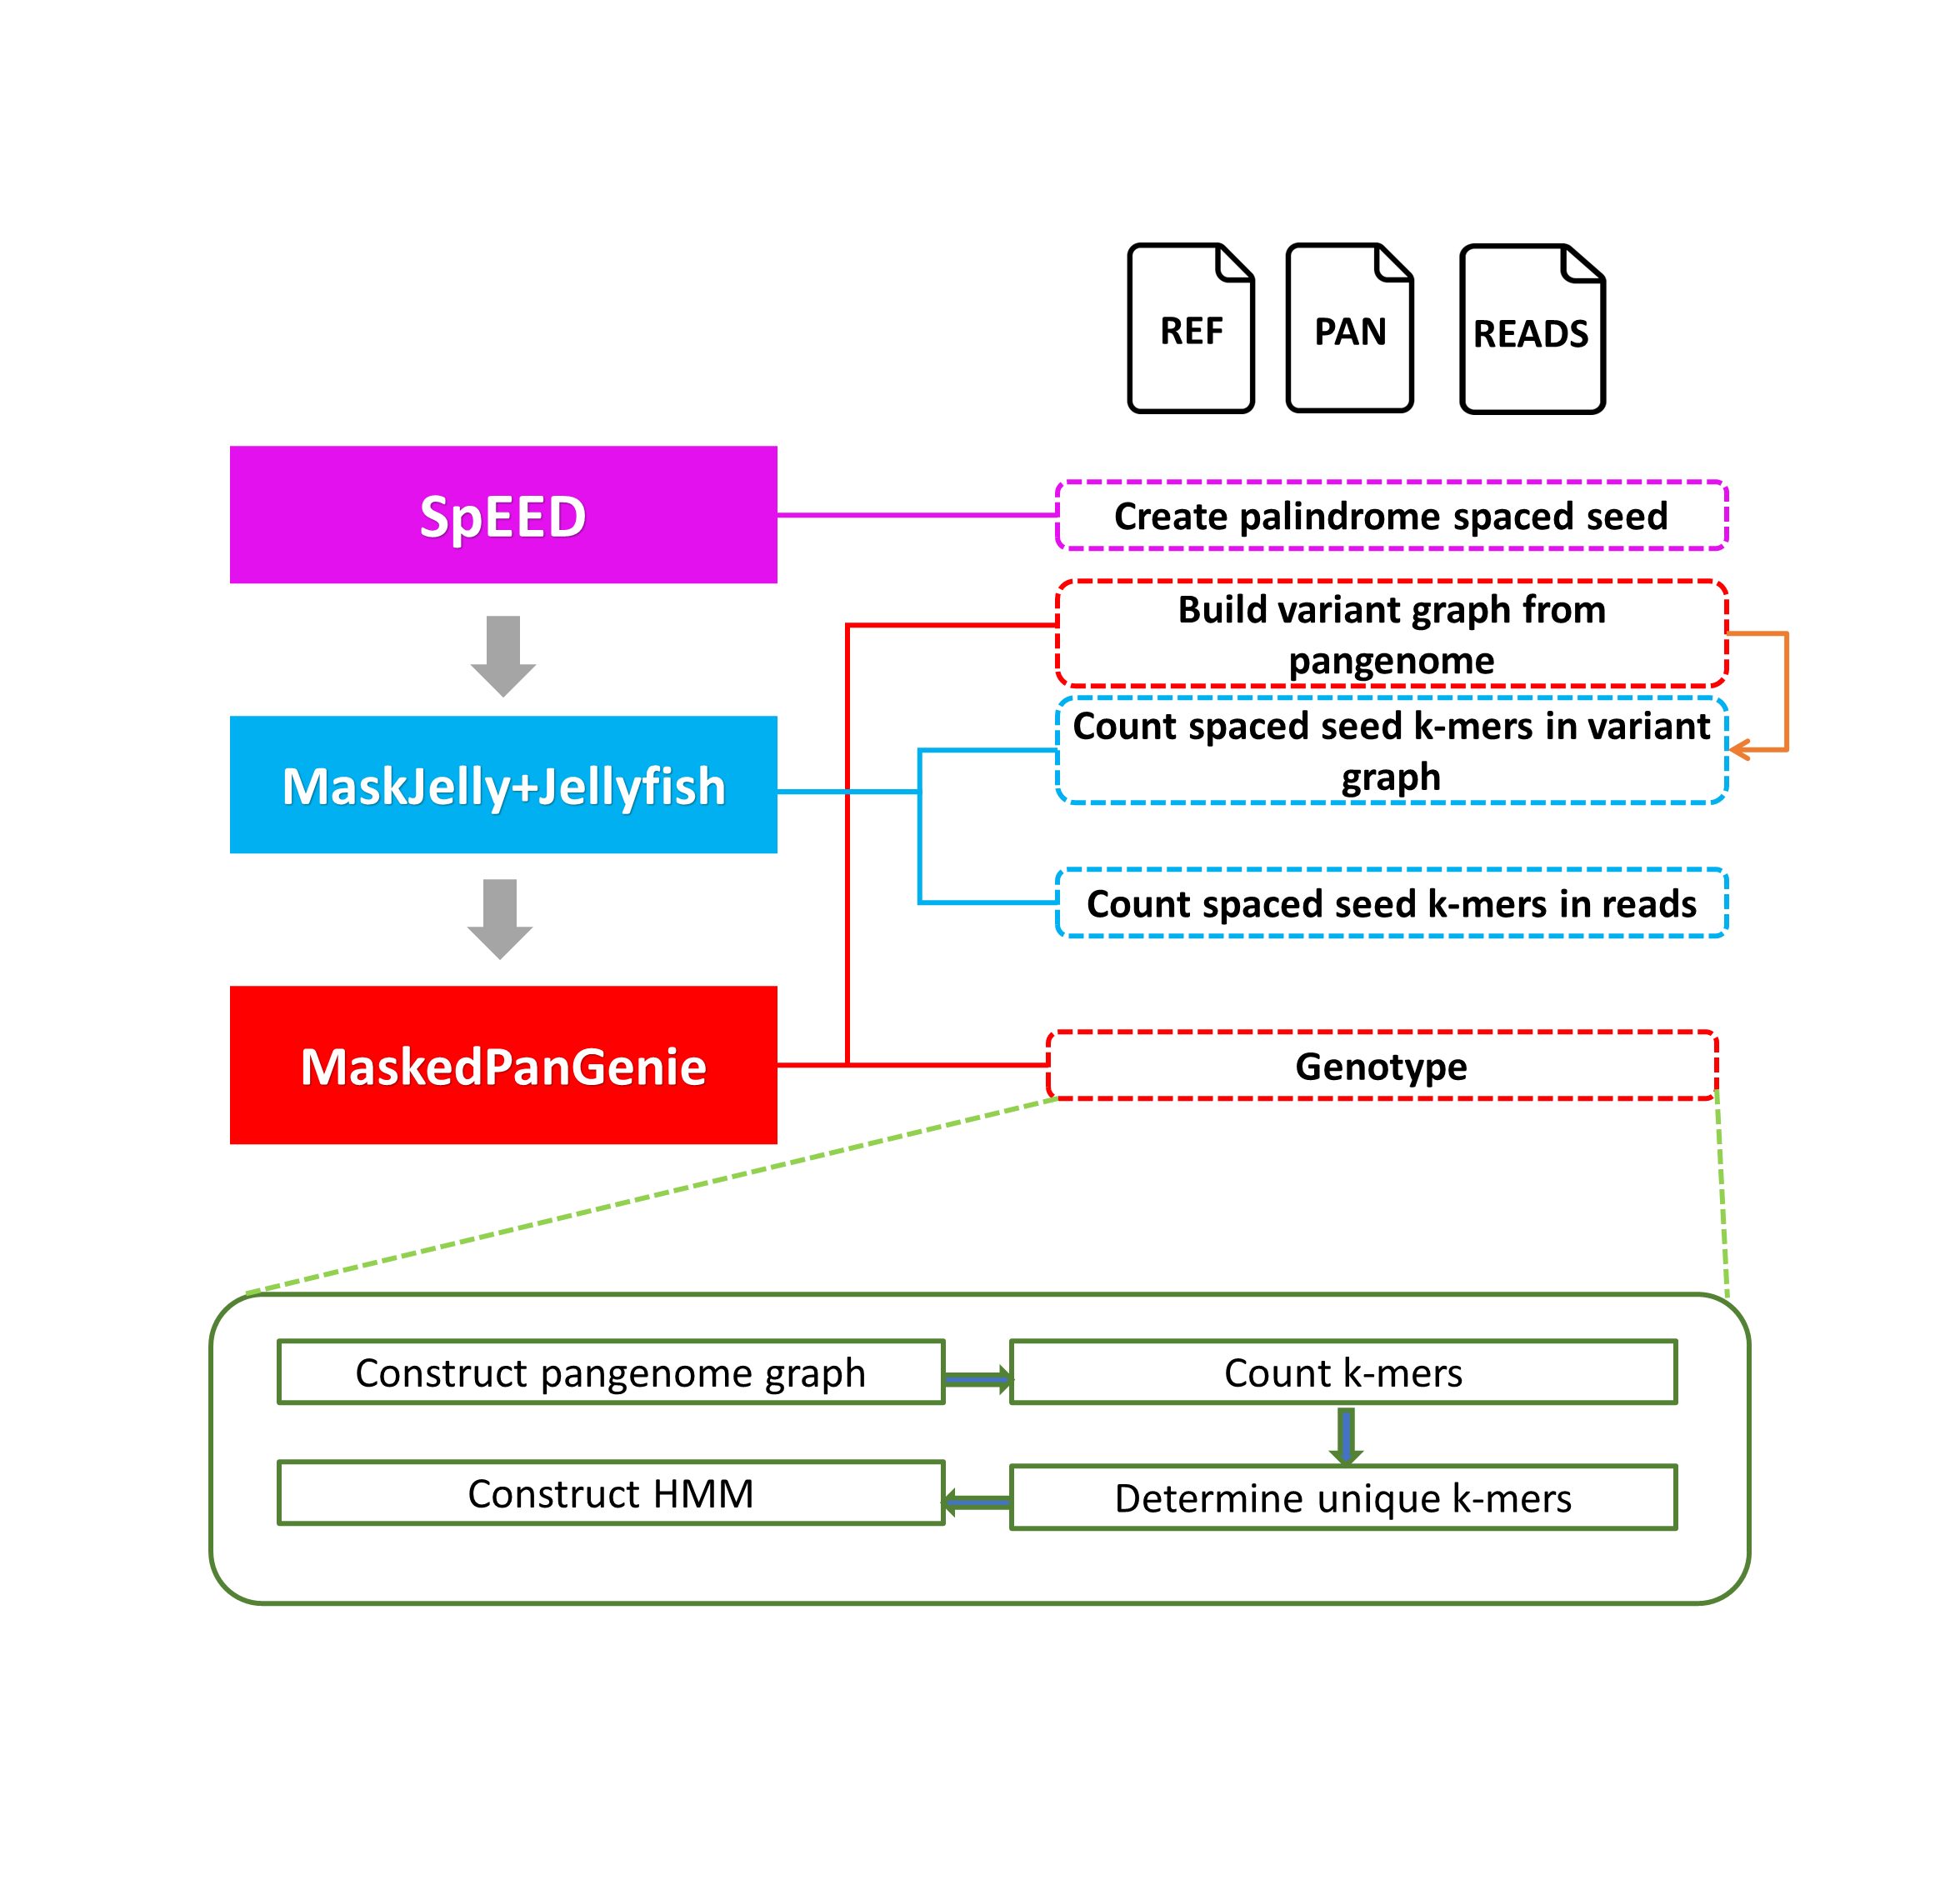
\includegraphics[scale=0.18]{figures/MaskedPanGenie_pipeline.png}
	\caption{Overview of MaskedPanGenie pipline}
	\label{fig:MaskedPanGenie} % \ref{this label}
\end{figure}

To obtain a palindrome spaced seed with a length of 51 and weight of 31, the authors first use the SpEED tool to obtain an approximate optimal spaced seed with a length of 26 and weight of 16. They then extend this seed by appending its mirrored version on the right side to ensure it is palindromic.

Before entering the genotyping phase, preprocessing is performed to enable the use of spaced seed for counting k-mers in the variant graph (built from the pangenome) and reads. This involves using the MaskJelly tool, which applies a spaced seed to a given fasta or jellyfish file and outputs the spaced k-mers. Jellyfish is then used to count the occurrences of these k-mers.

The processed files from the preprocessing stage are input into MaskedPanGenie for genotyping, which consists of the following four steps:
1. Construction of a pangenome graph based on the provided variant callset.
2. Utilizing the dictionaries generated during preprocessing, which contain the counts of spaced k-mers in reads and the pangenome graph.
3. MaskedPanGenie determines unique k-mers specific to a variant bubble in the pangenome. It applies the provided palindrome spaced seed to mask all k-mers of a variant bubble and compares the counts of spaced k-mers across the entire genome. If the counts are equal for a k-mer, it uniquely belongs to the tested variant bubble.
4. Creating and running a Hidden Markov Model (HMM) to predict the most likely genotypes for the sample.


\chapter{Research Methodology}
\section{PalindromeSpEED}
Although there are several software tools available today to calculate spaced seed sets with better sensitivity, including SpEED~\cite{Lucian2011SpEED} and Rasbhari~\cite{Hahn2016Rasbhari}, as far as I know, there is no direct support for computing the optimal palindrome spaced seeds. This is because spaced seeds are more widely used in similarity and sequence alignment analyses. However, MaskedPanGenie uses canonical representations of k-mers, allowing matching of corresponding loci even if the read originates from the reverse strand~\cite{haimo2023MaskedPanGenie}. To obtain a palindrome spaced seed (e.g., length 51, weight 31), the authors of MaskedPanGenie used the SpEED tool to optimize a length 26 weight 16 spaced seed through 4680 iterations and then extended it with its mirrored version to ensure palindromicity.

However, this approach does not guarantee the highest sensitivity for the obtained palindrome spaced seed pattern (with length 51 and weight 31). The SpEED tool has a maximum weight limit of 22 and does not allow setting the length. To address this, PalindromeSpEED, an algorithm based on SpEED, was developed to obtain better palindrome spaced seeds. The workflow is as follows:

Initially, a random palindrome spaced seed is generated based on user-defined length and weight. Then, through a series of iterations, optimization is performed. The optimization steps include randomly selecting two positions in the first half of the palindrome spaced seed where 1 and 0 combinations exist, flipping their values, and updating the corresponding positions in the second half to maintain the palindrome pattern. The overlap complexity of the modified palindrome spaced seed is calculated, and if it is lower than the current best overlap complexity, the modified seed becomes the new best result. This process continues for all possible combinations in the first half of the seed length, and the best flip results are used to modify the original palindrome spaced seed.

The modified palindrome spaced seed is evaluated for sensitivity. The sensitivity calculation utilizes the dynamic programming algorithm of Li et al.~\cite{Li2004PatternHunter2}, implemented in SpEED and Rasbhari tools, to calculate the spaced seed sensitivity with the given parameters. If the sensitivity of the modified palindrome spaced seed is higher than the current best sensitivity, it becomes the new best result. This process continues until the specified number of iterations is reached or until the user determines that a satisfactory palindrome spaced seed has been obtained, allowing for premature termination of the program. This approach improves the selection of palindrome spaced seeds with higher sensitivity for use in MaskedPanGenie.
\begin{algorithm}
    \caption{Pseudocode of the implementation for PalindromeSpEED}
    \label{alg:PalindromeSpEED}
    - given: the weight $w$, the length $l$, length of the homology region $n$, similarity level $p$, and iteration $t$
    \begin{algorithmic}
        % \State $S \gets \texttt{1s1s'1}\texttt{ with s'=reverse(s)}$
        \State $S \gets \texttt{PalindromeSpacedSeed}(l,w)$
        \For{$i=0$ ; $i \textless t$ ; $i++$}
            \While{OC(flip($S,k,j$)) < OC($S$) with $\{S[k],S[j]\} = \{1, 0\}$}
                \State choose a pair $(k, j)$ that minimizes OC(.)
                \State $S \gets \texttt{flip}(S,k,j)$
            \EndWhile
            \If{Sensitivity($S,n,p$) > BestSensitivity}
                \State $\texttt{BestSensitivity} \gets \texttt{Sensitivity}(S,n,p)$
            \EndIf
        \EndFor\\
        \Return $S$
    \end{algorithmic}
\end{algorithm}

PalindromeSpEED required parameters are palindrome spaced seed length (-l), length of the random region(-N), similarity level(-p),palindrome spaced seed weight(-w) as well as the optimization iteration(-t). Comparing the palindrome spaced seed generated by the original method and the PalindromeSpEED method(see Table \ref{table:PalindromeSpEED}), we observe that the PalindromeSpEED method demonstrates better sensitivity relative to the original method in two scenarios. In the first case, with a spaced seed length of 41 and weight of 31, and in the second case, with a spaced seed length of 39 and weight of 25.
\begin{table}[h!]
	\centering
	\begin{tabular*}{\textwidth}{@{\extracolsep{\fill}}ccc@{\extracolsep{\fill}}}
        \toprule
        Method & Palindrome Spaced Seed & Sensitivity\\
        \midrule
        Original&11101110110110101111111110101101101110111&0.826843\\
        Original&11111010110110111011111011101101101011111&0.838849\\
        PalindromeSpEED&11111110110101110011111001110101101111111&\textbf{0.856148}\\
        \midrule 
        Original&111010011010011101111101110010110010111&0.94561\\
        Original&111011100101100101111101001101001110111&0.955228\\
        PalindromeSpEED&111110110110001101010101100011011011111&\textbf{0.958913}\\
        \bottomrule 
	\end{tabular*}
	\caption{Palindrome spaced seed generated by the original method and the PalidromeSpEED.}
	\label{table:PalindromeSpEED}
\end{table}
\section{MaskedJellyfish}
Since the original version of Jellfish does not support spaced k-mer counting, the authors of MaskedPanGenie created a preprocessing tool called MaskJelly to enable the counting of spaced k-mers using Jellfish. However, this approach leads to an increase in overall runtime for two main reasons: 1. It requires reading the input file twice: once for the original FASTA file and again for the processed FASTA file. Although pipelines can be used to reduce disk I/O and temporary file creation, the actual cost remains high. 2. MaskJelly does not support multiple threads and has a simpler implementation compared to other tools.

To optimize the process, two options can be considered: modifying the source code of Jellfish or using alternative tools that support spaced k-mer counting. In this case, the chosen approach is to modify Jellfish's source code, as it allows for seamless integration with the MaskedPanGenie software, as discussed in subsequent chapters. The modification was made to Jellfish version 2.3.0(\url{https://github.com/gmarcais/Jellyfish}), which offers improved efficiency and includes a Bloom filter-based mode for removing singleton k-mers (k-mers occurring only once in the dataset). MaskedPanGenie utilizes a modified version of the jellyfish2 library for k-mer counting.

Before delving into the modifications, it's important to understand two challenges that arise:
1. If we directly select spaced seeds for each k-mer (e.g., from 51-mers to 31-mers), Jellfish automatically discards any k-mers that contain "N" symbols. Consequently, if the original FASTA file contains sequence errors (typically represented by "N"), the information around those "N" symbols is lost. However, spaced seeds have the potential to mask "N"-containing k-mers and retrieve valuable information (e.g., k-mers with variant sequence). Therefore, we cannot directly use Jellfish's built-in k-mer counting approach to handle spaced seeds.
2. In Jellfish's file reading process, an "N" is added after each sequence to mark the start of a different sequence. If we only encode "N" as a symbol (e.g., A=0, C=1, G=2, T=3, N=4), errors occur during k-mer counting because "N" represents either a sequence error or the end of a sequence.

To address these challenges, the modifications involve processing the sequences for spaced seeds before inserting them into Jellfish's buffer. The modified approach follows Jellfish's method of handling different sequences and appends an "N" to the end of each spaced k-mer. Additionally, a reference FASTA file is utilized, where each sequence represents a chromosome. An additional space is allocated to copy the final k-mer, as long sequences (exceeding the predetermined limit, typically 200 bp) cannot be processed at once. This copying method ensures that the entire read is properly processed even if it extends beyond the set limit.
\subsubsection{FSH\cite{Girotto2018FSH} algorithm applied in MaskedPanGenie}
The FSH (Fast Spaced Seed Hashing Exploiting Adjacent Hashes) algorithm is employed to address the process of applying spaced seeds to genomic sequences in MaskedPanGenie. Spaced seed masking involves extracting specific sub-patterns from each read k-mer, such as removing certain positions based on the mask pattern (e.g., ATAACCT with a spaced seed of 1101100 becomes ATAC). However, this straightforward approach is slower compared to handling contiguous k-mers due to the shared subsequence property of contiguous k-mers.

To optimize the runtime efficiency, the FSH algorithm is introduced to reduce the number of symbol copies and improve overall performance. The idea behind FSH is to utilize the previous k-mer set that can provide the maximum number of shared symbols at the same positions. This is achieved by defining $Cj = \{i-j\in Q:i\in Q \wedge m(i-j) = m(i) - m(j) \}$ as the positions in Q that remain in Q after j shifts, where j < s(Q) and m(k - j) = m(k) - m(j).

By applying the FSH algorithm, we can add only $\left|Q\right|-\left|C_j\right|$ symbols at positions $Q\textbackslash C_j$. However, it was observed that the overall runtime improvement was not substantial compared to the original approach. This could be attributed to two main factors: 1.The FSH algorithm does not consider the presence of "N" symbols, requiring additional time to handle these cases compared to the original algorithm, which can handle them directly. 2.The FSH algorithm involves preprocessing to determine the best positions of previously known k-mers during the traversal of the sequence. This optimization aims to reduce the number of symbols that need to be read. However, the overhead generated by this preprocessing step impacts the final runtime results.

Although further acceleration was not achieved, MaskedJellyfish is already a noticeable improvement compared to the combination of MaskJelly and the Jellyfish tool.
\section{MaskedPanGenie}

Before understanding the approach, we need to explain the reasons behind the high runtime of the original MaskedPanGenie pipeline compared to the PanGenie tool:

MaskedPanGenie requires additional time for preprocessing, which includes the following steps:
1.Building a variant graph from the pangenome. 2.Counting spaced seed k-mers in the variant graph. 3.Counting spaced seed k-mers in the reads. Only after these preprocessing steps, the processed reads and pangenome jellyfish files, along with the reference.fasta and pangenome.vcf, are used as input to MaskedPanGenie. According to the original author's runtime tests, the preprocessing step alone accounts for more than half of the total MaskedPanGenie runtime, making it a significant time-consuming process.

Additionally, identifying unique k-mers in MaskedPanGenie also requires more time. This is due to the lack of safe multi-threaded access support for k-mer dictionaries in Jellyfish's implementation within MaskedPanGenie~\cite{haimo2022issue}. As a result, the author used mutexes to guard the dictionaries, ensuring deterministic behavior. However, using mutex locks introduces additional time overhead. This includes the need for thread synchronization and potential performance degradation when multiple threads contend for the same resource, as other threads have to wait for the execution thread to release the resource.

Given these reasons, we need to modify MaskedPanGenie to address both issues. I modified the software "MaskedPanGenie," written in C++, available at \url{https://github.com/hhaentze/MaskedPangenie}.

The main modifications are made in the following two parts: 1.Counting k-mers in reads and the pangenome graph. 2.Determining unique k-mers. In the first part, "Counting k-mers in reads and the pangenome graph," we include the MaskedJellyfish library to enable spaced k-mer counting for reads and the pangenome graph. This modification eliminates the need for additional preprocessing time, allowing MaskedPanGenie to directly count the occurrence of those k-mers using the original reads.fasta, pangenome.vcf, and ref.fasta, similar to the parameters used in PanGenie execution.

In the second part, "Determining unique k-mers," we remove the mutex lock approach previously used by the original authors to handle multi-threaded access to Jellyfish k-mer dictionaries. This is possible because of the modifications made in the first part, enabling MaskedPanGenie to perform spaced k-mer counting in a multi-threaded environment. Therefore, MaskedPanGenie can now utilize a provided spaced seed to mask all k-mers of a variant bubble and compare the counts of spaced k-mers instead.

To summarize, this approach effectively reduces the overall runtime and simplifies the MaskedPanGenie pipeline (Figure \ref{fig:MaskedPanGenie_revised}) by eliminating the preprocessing step. The required parameters include the sequencing reads in FASTA/FASTQ format (-i), the variant callset (-v), the reference sequence (-r), and the spaced seed used for creating the dictionaries.
\begin{figure}
	\centering
	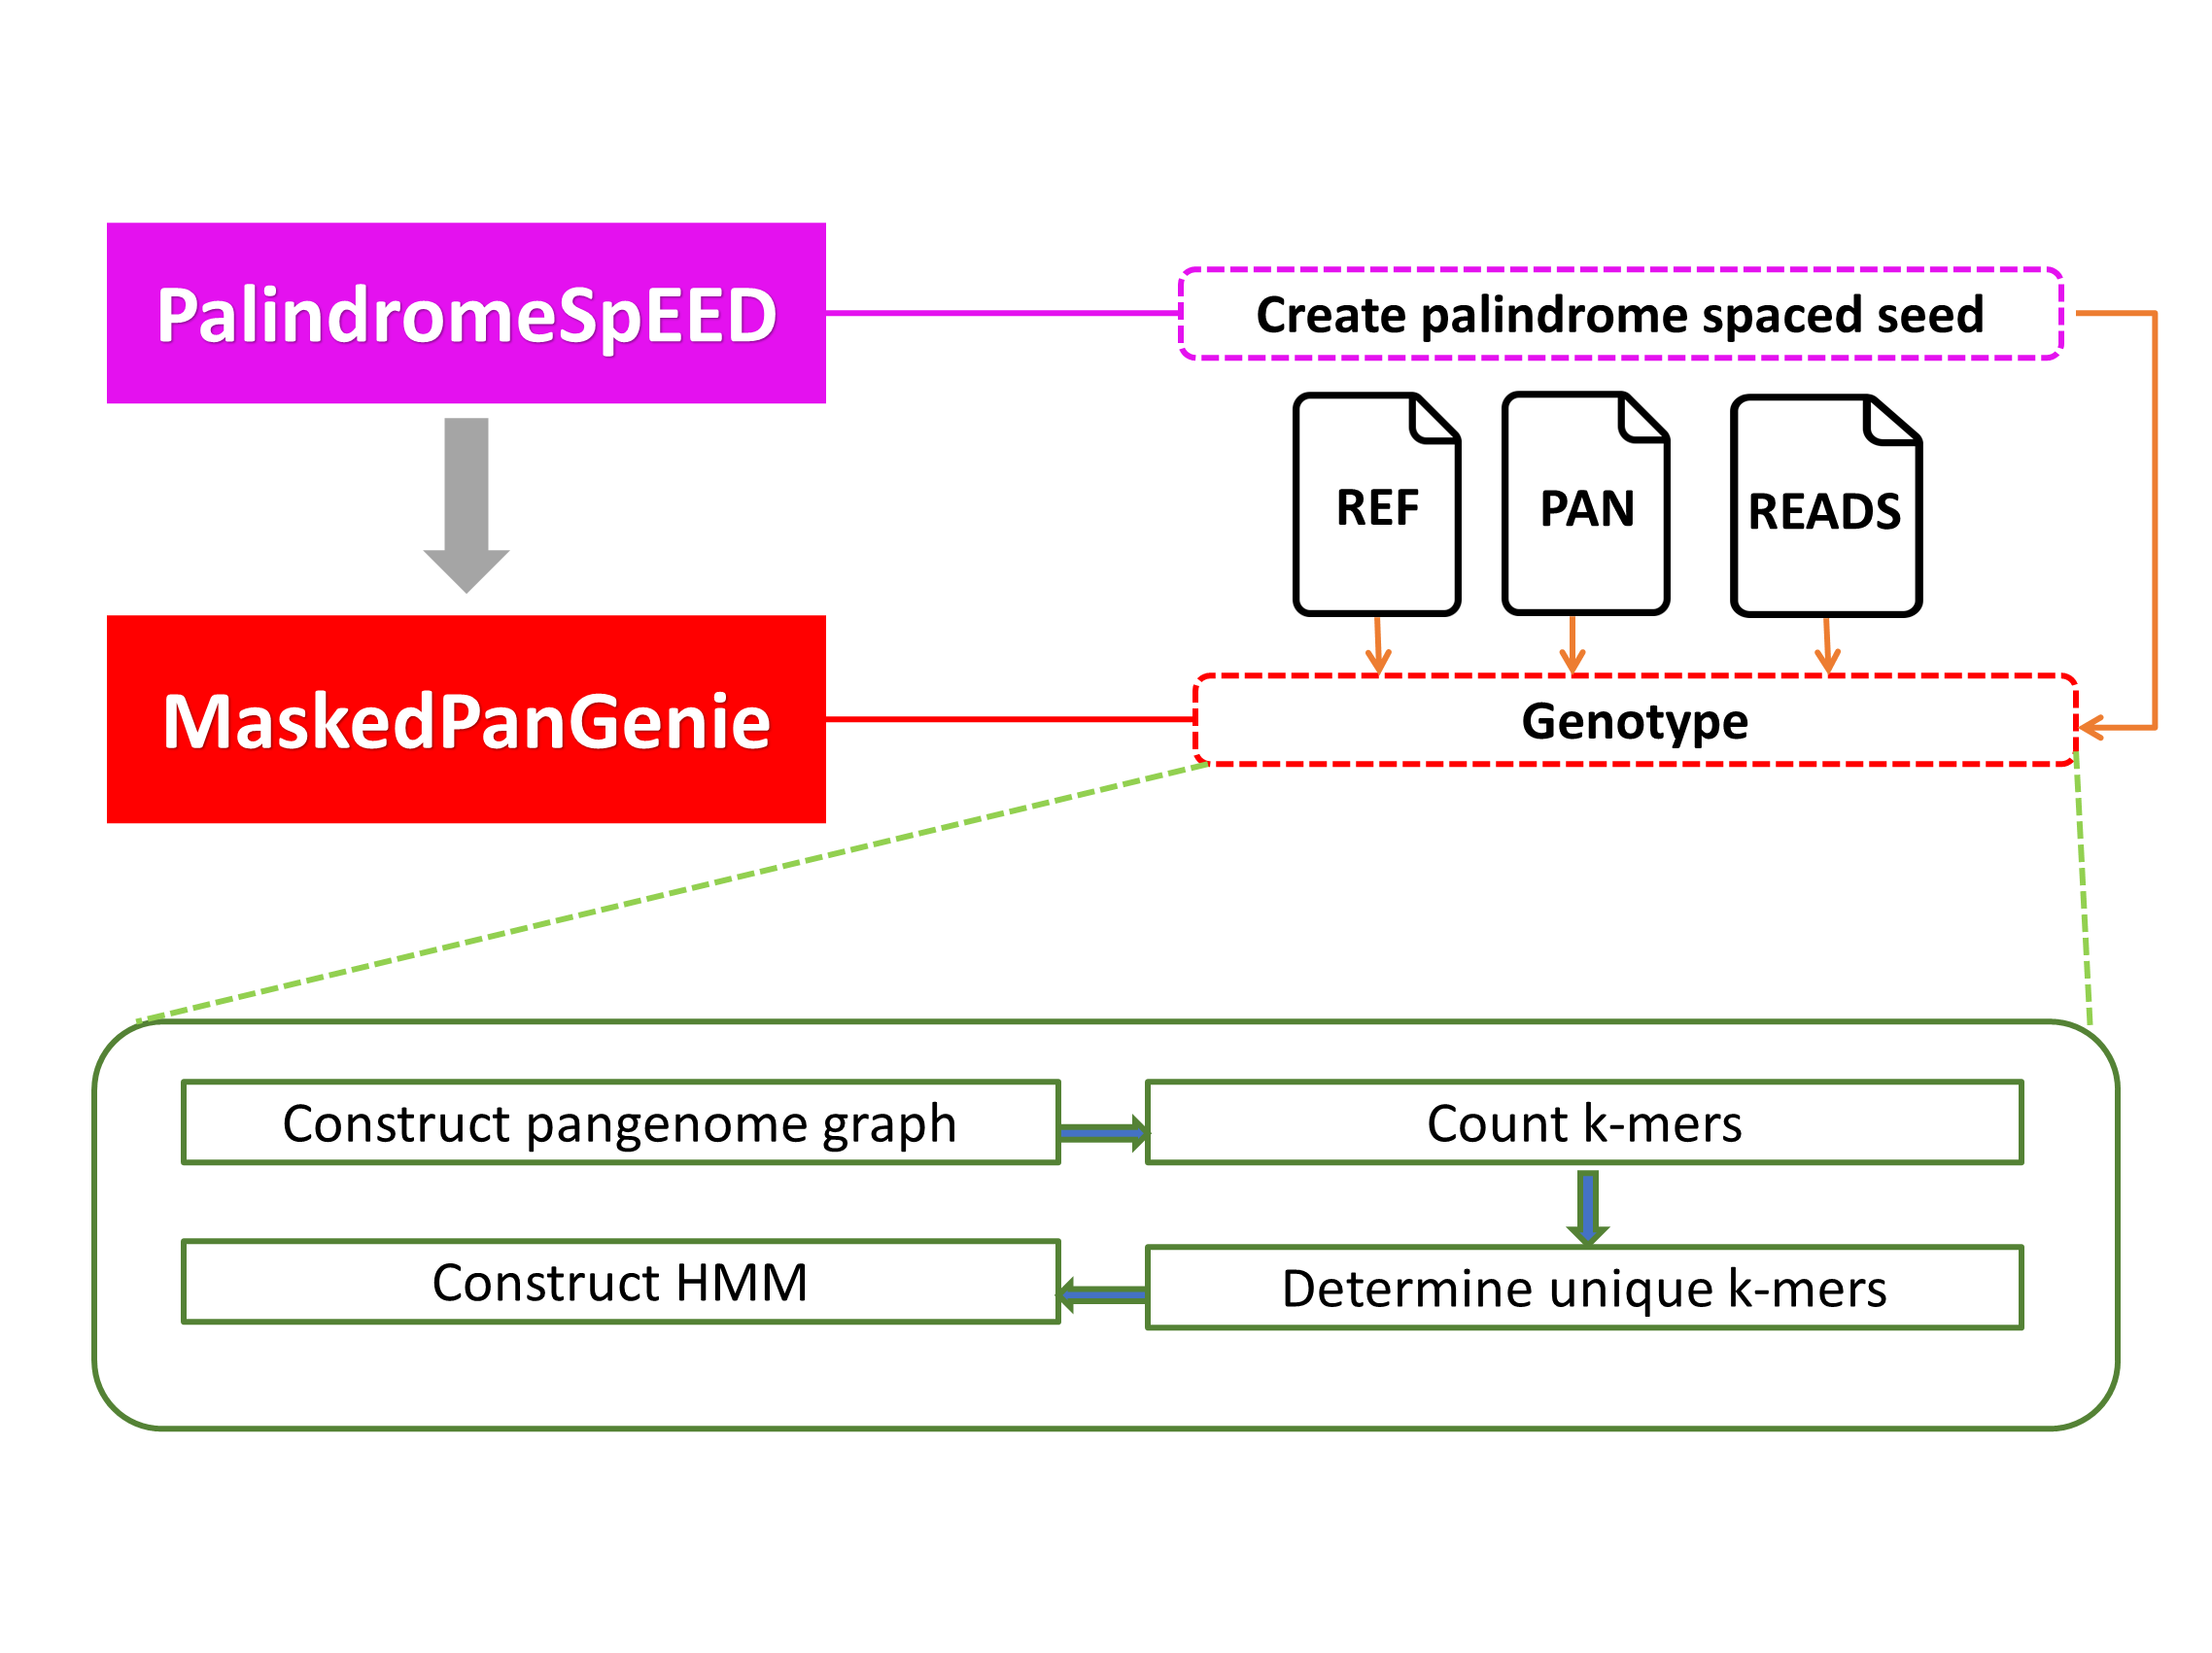
\includegraphics[scale=0.18]{figures/MaskedPanGenie_revised.png}
	\caption{MaskedPanGenie pipline}
	\label{fig:MaskedPanGenie_revised} % \ref{this label}
\end{figure}
\chapter{Data}
\section{Pangenome reference}
In this study, the haplotype-resolved pangenome graph was constructed using data from 11 unrelated individuals, specifically NA19238, NA19239, HG00731, HG00732, HG00512, HG00513, NA12878, HG02818, HG03125, NA24385, and HG03486, as reported by Hartmut Häntze~\cite{haimo2023MaskedPanGenie}. The author merged variation calls and filtered for variants shared by at least one of the 11 samples, where the alternative genotype of at least 80\% of the samples is known. The number of variants covered by the pangenome graph was reported based on Hartmut Häntze's report~\cite{haimo2023MaskedPanGenie}.

For the leave-one-out cross-validation, subsets of the pangenome were used, excluding the haplotypes of the tested individual. These excluded haplotypes were considered as the ground truth. Variants not covered by the true haplotype of the tested individual or the remaining haplotypes in the pangenome were removed from the analysis.
\section{Reads}
The test data consisted of reads from nine selected individuals out of the eleven individuals used to build the pangenome reference. All reads were sequenced within the same BioProject using an Illumina HiSeq X Ten system with a whole-genome sequencing strategy, a coverage of 30x, and paired layout. The two remaining individuals were not part of the BioProject and were excluded from this study's workflow to avoid potential noise introduced by different sequencing platforms. The specific individuals and their corresponding sequence read archive (SRA) accessions are provided, along with their ancestral backgrounds.
\begin{itemize}
    \item HG00731: SRR7782675(Puerto Rico - American Ancestry, Male)
    \item HG00732: SRR7782676(Puerto Rico - American Ancestry, Female)
    \item HG00512: SRR7782672(Han Chinese - East Asian Ancestry, Male)
    \item HG00513: SRR7782673(Han Chinese - East Asian Ancestry, Female)
    \item NA19238: SRR7782690(Nigeria - African Ancestry, Female)
    \item NA19239: SRR7782691(Nigeria - African Ancestry, Male)
    \item NA12878: SRR7782683(Utah - European Ancestry, Female)
    \item HG02818: SRR7782682(The Gambia - African Ancestry, Female)
    \item NA24385: SRR7782670(Ashkenazim Jewish Ethnicity, Male)
\end{itemize}

To assess the impact of spaced seeds on reads with lower coverage, the author sampled the reads down to a target coverage of 5x. The DownsampleSam approach was used, which includes randomly sampling reads that could not be aligned to the reference genome to the same fraction.

\chapter{Results}

\section{Spaced k-mer counting}
We compare the runtime of MaskedJellyfish to the original approach of using MaskJelly+Jellyfish for counting spaced k-mers. Tests were executed on a Linux server with a single AMD $\texttt{Ryzen}^{\texttt{TM}}$ 9 5950X desktop processor, consisting of 16 hyper-threaded physical cores running at their base clock 3.4GHz, and 128 GB of random access memory. This section, we will consider two scenarios: 1.Time taken for different CPU threading settings. 2.Runtime on the original MaskedPanGenie preprocessing step.
\begin{itemize}
    \item Spaced Seed used: 11111110101001110001011001001101000111\\0010101111111(length = 51, weight = 31)
\end{itemize}
\subsection{Time taken for different CPU threading settings} 
We wanted to compare the runtime of MaskedJellyfish with the original method (MaskJelly + Jellyfish) for calculating spaced k-mer counting. The motivation behind this comparison was that the original MaskJelly does not support multithreaded environments. We speculated that the two methods would exhibit significant time differences when varying the number of threads since MaskedJellyfish supports multithreading. We used the dataset M\_abscessus\_HiSeq\_10M.f-asta, which consisted of 2.5 million pairs of 100bp reads sampled from the HiSeq M. abscessus 6G-0125-R dataset in GAGE-B.

The results (Fig \ref{fig:thread_compare}) showed that MaskedJellyfish exhibited a noticeable decrease in runtime compared to the original MaskJelly + Jellyfish method, with a speedup of at about 2 times. However, there was no significant time difference observed due to multithreading in MaskedJellyfish, contrary to our initial speculation. To investigate this further, we conducted experiments by fixing the thread count to 16 for Jellyfish and observing the runtime of MaskJelly under different thread settings.

From the resulting graph (Fig \ref{fig:MaskJelly_thread}), it became evident that MaskJelly does offer multithreading functionality, as there were noticeable time differences observed when using different thread counts. This explains why we couldn't observe the impact of multithreading in the original graph. In conclusion, the MaskedJellyfish method showed significant improvement in runtime compared to the original method for calculating spaced k-mer counting.
\begin{figure}
	\centering
	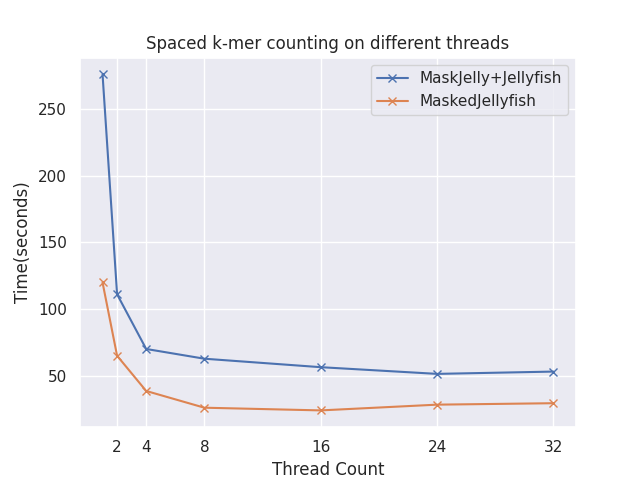
\includegraphics[scale=0.7]{figures/M_compare.png}
	\caption{Execution time for spaced k-mer counting on two methods}
	\label{fig:thread_compare} % \ref{this label}
\end{figure}
\begin{figure}
	\centering
	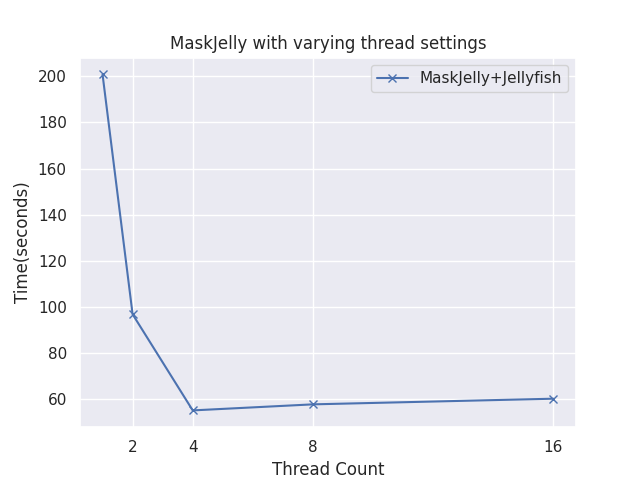
\includegraphics[scale=0.7]{figures/MaskJelly_thread.png}
	\caption{Execution time for MaskeJelly on different numbers of threads and Jellyfish count for 16 threads}
	\label{fig:MaskJelly_thread} % \ref{this label}
\end{figure}

\subsection{Runtime on preprocessing step}
We focuses on the preprocessing step in the original MaskedPanGenie pipeline, where spaced k-mer counting is performed on the variant graph and reads using 16 threads. We compare the runtime of both methods using the dataset "NA12878" with 30-fold coverage. Afterwards, We will summary and Comparison of Overall Runtime in MaskedPanGenie. The preprocessing step can be divided into the following parts:
\begin{enumerate}[label=(\roman*)]
\item Build variant graph from the pangenome.
\item Count spaced seed k-mers in the variant graph (spaced k-mer counting).
\item Dump jellfish file to a fasta file.
\item Count spaced seed k-mers in the reads (spaced k-mer counting).
\end{enumerate}
From the results (Table \ref{table:MaskedJellyfish}), it is observed that using the MaskedJellyfish method significantly reduces the time required for calculating spaced k-mer counting in parts (ii) and (iv) of the preprocessing step, achieving a 2x speed improvement compared to the original method. However, for the overall time of the MaskedPanGenie pipeline, the speed improvement is only 1.5x. It was also found that both methods require equal time for parts (i) and (iii), which means that even with continued optimization of the spaced k-mer counting algorithm, these parts still require a significant amount of time. This led to the proposed modification of the MaskedPanGenie method, which eliminates the need for the preprocessing step in comparison to the PanGenie workflow, allowing direct utilization of the jellyfish library for k-mer counting during the genotyping stage.
\begin{table}[ht!]
	\centering
	\begin{tabular*}{\textwidth}{@{\extracolsep{\fill}}ccccccc@{\extracolsep{\fill}}}
        \toprule
         & (i) & (ii) & (iii) & (iv) & MaskedPanGenie & Total\\
         Method & & & & & &\\
        \midrule
        MaskJelly+Jellyfish& 8 min & \textbf{20 min} & 30 min & \textbf{292 min} & 2h:52min & 8h:42min\\
        MaskedJellyfish& 8 min & \textbf{10 min} & 30 min & \textbf{102 min} & 2h:52min & 5h:28min\\
        \bottomrule 
	\end{tabular*}
	\caption{The runtime comparison of MaskJelly+Jellyfish and MaskedJellyfish for spaced k-mer counting in the preprocessing step of the NA12878 sample with 30-fold coverage.}
	\label{table:MaskedJellyfish}
\end{table}
\section{MaskedPanGenie pipeline}
We compared the revised MaskedPanGenie pipeline, which eliminates the preprocessing step, with the original MaskedPanGenie pipeline, which includes the preprocessing step. The tests were conducted on a Linux server equipped with a single Intel(R) Xeon(R) Gold 6242 processor, featuring 16 hyper-threaded physical cores operating at 2.8GHz, and 128 GB of random access memory.
\begin{itemize}
    \item Spaced Seed used: 11111110101001110001011001001101000111\\0010101111111(length = 51, weight = 31)
\end{itemize}
\subsection{Runtime comparison}
The dataset used for evaluation was NA12878 with 30-fold coverage. In the context of MaskedPanGenie~\cite{haimo2023MaskedPanGenie}, the genotyping step can be further divided into four sections:
\begin{enumerate}[label=(\roman*)]
\item Construction of a pangenome graph based on a provided VCF file.
\item Counting k-mers in reads and the pangenome graph.
\item Determining unique k-mers.
\item Constructing an HMM (Hidden Markov Model) and calculating the most likely genotypes.
\end{enumerate}
The results in Table \ref{table:MaskedPanGenie} demonstrate a notable reduction in runtime for the revised MaskedPanGenie compared to the original MaskedPanGenie with preprocessing step. This improvement is primarily attributed to significant time savings in the preprocessing step and HMM step, resulting in an overall speedup of over 2x compared to Häntze's MaskedPanGenie. The primary factors contributing to this improvement are as follows:

Firstly, the preprocessing step, which was the main target of modification, plays a crucial role in saving time and simplifying the pipeline. Instead of performing spaced seed processing beforehand, the revised pipeline integrates it into the second step, i.e., counting k-mers in reads and the pangenome graph. Consequently, the revised MaskedPanGenie exhibits longer runtime in the counting step compared to the original version.

Secondly, the section for determining unique k-mers (iii) has been optimized in the revised MaskedPanGenie. The original approach, although accurate, employed more time-consuming methods. In contrast, the revised MaskedPanGenie employs a faster version while still maintaining the accuracy.

The analysis of this performance comparison provides valuable insights into the benefits of the revised MaskedPanGenie pipeline. By eliminating the preprocessing step and enhancing the efficiency of spaced k-mer counting, the revised pipeline offers faster and more streamlined genomic analyses, simplifying the overall workflow.
\begin{table}[ht!]
	\centering
	\begin{tabular*}{\textwidth}{@{\extracolsep{\fill}}ccccccc@{\extracolsep{\fill}}}
        \toprule
         & Pre- & Reading & Counting & Unique & HMM & Total\\
         Method & processing & Input & & & &\\
        \midrule
        MaskedPanGenie(i)& 5h:50min & 11min & 2min & 65min & 94min& 8h:42min \\
        MaskedPanGenie(ii)& 2h:30min & 11min & 2min & 65min & 94min & 5h:28min\\
        MaskedPanGenie(iii)& - & 11min & 1h:4min & 4min & 94min & \textbf{2h:53min}\\
        \bottomrule 
	\end{tabular*}
    \caption{The runtime comparison for genotyping NA12878 with 30-fold coverage between Häntze's MaskedPanGenie(i), MaskedJellyfish+MaskedPanGenie (ii), and the Revised\_MaskedPanGenie (iii).}
	\label{table:MaskedPanGenie}
\end{table}
\subsection{Memory comparison}
The testing dataset used was the "chapter 4 Data" for HG00512, HG00731, NA12878 and NA19238 with 30-fold coverage, consisting of four read datasets. From the results (Table \ref{table:Space_MaskedPanGenie}), it is evident that the revised MaskedPanGenie pipeline exhibits a significant reduction in memory usage compared to the original MaskedPanGenie pipeline. The primary reason for this is as follows:

In the original MaskedPanGenie version, a preprocessing step is required to perform spaced k-mer counting. This preprocessing step generates processed data, which is then used as input for MaskedPanGenie along with the original data. As a result, more memory space is required to accommodate both the processed data and the original data.

However, in the revised MaskedPanGenie, there is no need to process the data separately before performing spaced k-mer counting. Instead, the pipeline utilizes the original data directly for calculating spaced k-mer counting. This eliminates the need for additional memory space to store processed data, resulting in more efficient memory usage.

\begin{table}[ht!]
	\centering
	\begin{tabular*}{\textwidth}{@{\extracolsep{\fill}}ccccc@{\extracolsep{\fill}}}
        \toprule
         & HG00512 & HG00731 & NA12878 & NA19238 \\
         Method & & & & \\
        \midrule
        MaskedPanGenie(i)& 93.9492GB & 94.5024GB & 93.9314GB & 93.6342GB\\
        MaskedPanGenie(ii)& 80.0799GB & 80.2827GB & 80.2818GB & 79.6233GB\\
        \bottomrule 
	\end{tabular*}
	\caption{Comparison of memory usage between the Häntze's MaskedPanGenie(i) and the revised MaskedPanGenie(ii) from four samples.}
	\label{table:Space_MaskedPanGenie}
\end{table}

\section{Spaced seed on genotyping}
The impact of spaced seed patterns on genotyping is analyzed in this study using MaskedPanGenie on reads with 5-fold and 30-fold coverage from nine samples. We examine the following three scenarios to understand how spaced seed patterns affect genotyping results and provide insights for users to select appropriate spaced seed patterns in MaskedPanGenie:
\begin{enumerate}
    \item Sensitivity: We evaluate the impact of sensitivity values (at the same length and weight) on the genotyping results.
    \item Care position: We compare the effect of the number of care positions (at the same length) on the genotyping results.
    \item Length variation: We examine how different lengths (at the same weight) of spaced seed patterns influence the genotyping results.
\end{enumerate}
By analyzing these scenarios, users can make informed decisions when choosing suitable spaced seed patterns in MaskedPanGenie for their genotyping needs.
\subsection{Sensitivity}
In this section, we aimed to investigate the impact of sensitivity values on the final genotyping results using different spaced seed patterns. Specifically, we set the spaced seed pattern (Table \ref{table:Sensitivity}) with a length of 51 and weight of 31, along with two additional contiguous seed patterns with lengths of 31 (seed0) and 51 (seed6). Among the spaced seed patterns, seed2 corresponds to the spaced seed used by the original author, while the other spaced seed patterns were generated using the PalindromeSpEED software and seed5 is the best palindrome spaced seed.

In this study, we not only aimed to validate the superiority of spaced seed patterns over contiguous seed patterns in achieving better genotyping results but also examined the effect of higher sensitivity values in the spaced seed patterns on the overall performance. Our findings indicate that spaced seed patterns, particularly those with higher sensitivity values, tend to yield improved genotyping results compared to contiguous seed patterns.

Table \ref{table:sensitivity-5x} and Table \ref{table:sensitivity-30x} present the genotyping results at 5-fold and 30-fold coverage, respectively. Figure \ref{fig:sensitivity_genotyping_5x} and Figure \ref{fig:sensitivity_genotyping_30x} illustrates the results of genotyping different variant types at various coverage levels for each seed. Based on the information provided, it can be observed that the spaced seed approach generally outperforms the contiguous seed approach. Moreover, spaced seeds with higher sensitivity (e.g., seed3, seed4, and seed5) tend to yield better genotyping results compared to seeds with lower sensitivity (e.g., seed1 and seed2).

\begin{table}[ht!]
    % \setlength{\abovecaptionskip}{0cm}
    % \setlength{\belowcaptionskip}{0pt}
    \centering
    \begin{tabular}{|c|c|c|}
    \hline
      Seeds&Seeds Pattern&Sensitivity\\
     \hline
         seed0&1111111111111111111111111111111(k31)&0.624134\\
    \hline
        seed1&001000010100101111111111111111111111101001010000100(worst)&0.614292\\
    \hline 
        seed2&000110001110100111101111111111101111001011100011000&0.714743\\
    \hline
        seed3&111011100101010011010011111110010110010101001110111(the author)&0.845999\\
    \hline
        seed4&111101010011100100110101111101011001001110010101111&0.846579\\
    \hline
        seed5&111111101010011100010110010011010001110010101111111(best)&0.860626\\
    \hline
        seed6&111111111111111111111111111111111111111111111111111(k51)&0.16447\\
    \hline
    \end{tabular}
    \caption{Seeds pattern and sensitivity - same length and same weight}
    \label{table:Sensitivity}
\end{table}
\subsection{Care position}
In this section, we compare the impact of different weighted spaced seed patterns on genotyping results at the same length. Table \ref{table:Care position} is set with a length of 51, where the weights of the seeds are as follows: seed0 (weight=21), seed1 (weight=31), seed2 (weight=41), seed3 (weight=51). It is important to note that the sensitivity of seed0 cannot be calculated. This is due to the fact that calculating sensitivity requires more time and additional memory resources for computation. However, due to limited memory resources, the generation of seed0 is based on the spaced seed generated by the PalindromeSpEED tool with the best overlap complexity.

Table \ref{table:care-5x} and Table \ref{table:care-30x} respectively display the genotyping results for each variant type (wGC, Precision, Recall, and F-score) at 5x coverage and 30x coverage. Figure \ref{fig:care_genotyping_5x} and Figure \ref{fig:care_genotyping_30x} illustrates the precision and recall for each seed in the genotyping results across different coverage levels and variant types. The results indicate that, at 5x coverage, a lower number of care positions leads to better genotyping results. However, in the case of 30x coverage, this trend is reversed for the snv variant type. 
\begin{table}[ht]
    % \setlength{\abovecaptionskip}{0cm}
    % \setlength{\belowcaptionskip}{0pt}
    \centering
    \begin{tabular}{|c|c|c|}
    \hline
      Seeds&Seeds Pattern&Sensitivity\\
    \hline
        seed0&110010010100010100001001111100100001010001010010011&X\\
    \hline
        seed1&111111101010011100010110010011010001110010101111111&0.860626\\
    \hline
        seed2&111111110111100101111110111011111101001111011111111&0.589374\\
    \hline
        seed3&111111111111111111111111111111111111111111111111111&0.16447\\
    \hline
    \end{tabular}
    \caption{Seeds pattern and sensitivity - same length and different weight}
    \label{table:Care position}
\end{table}

\subsection{Length variation}
In this section, we evaluate the impact of varying the length of spaced k-mers on genotyping results. Table \ref{table:Length variation} is presented with a fixed weight of 31 and k-mer lengths ranging from seed0 (length = 31) to seed3 (length = 61). It should be noted that the sensitivity for seed3 cannot be calculated for the same reasons mentioned in the previous section. Therefore, we chose the length of 61 and weight of 31 as the spaced seed with the best overlap complexity for genotyping.

% Determining the appropriate length of k-mers is a crucial factor in various computational analyses, including genotyping. The choice between shorter and longer k-mers involves trade-offs and considerations. Shorter k-mers, typically ranging from 15 to 31 base pairs, offer advantages such as increased sensitivity and specificity in sequence matching. They can effectively capture local similarities and variations within a genome or sequence dataset. Short k-mers are particularly useful for identifying short sequence motifs, detecting small variations, and distinguishing closely related sequences. On the other hand, longer k-mers, typically exceeding 31 base pairs, provide a broader context and capture more global patterns within a sequence. They offer higher sequence specificity and can better handle repetitive regions and larger genomic variations. Longer k-mers are beneficial when analyzing complex genomes, identifying large structural variations, or distinguishing distantly related sequences.

The genotyping results from Table \ref{table:len-5x}, Table \ref{table:len-30x}, Figure \ref{fig:len_genotyping_5x} and Figure \ref{fig:len_genotyping_30x} consistently demonstrate that longer k-mer lengths yield better overall genotyping performance. However, an interesting observation is that this trend is reversed for precision, which is contrary to what was expected based on previous findings mentioned in MaskedPanGenie~\cite{haimo2023MaskedPanGenie}. The authors of MaskedPanGenie acknowledge this discrepancy but are uncertain about the underlying reasons for not observing this trend in their data.
\begin{table}[ht]
    % \setlength{\abovecaptionskip}{0cm}
    % \setlength{\belowcaptionskip}{0pt}
    \centering
    \begin{tabular}{|c|c|c|}
    \hline
      Seeds&Seeds Pattern&Sensitivity\\
    \hline
        seed0&1111111111111111111111111111111&0.624134\\
    \hline
        seed1&11111110110101110011111001110101101111111&0.856148\\
    \hline
        seed2&111111101010011100010110010011010001110010101111111&0.860626\\
    \hline
        seed3&1111000110010100101000100110111110110010001010010100110001111&X\\
    \hline
    \end{tabular}
    \caption{Seeds pattern and sensitivity - different length and same weight}
    \label{table:Length variation}
\end{table}

\begin{table*}[ht!]
\begin{tabular*}{\textwidth}{@{\extracolsep{\fill}}llllll@{\extracolsep{\fill}}}
\toprule
   &         &               wGC &         Precision &            Recall &           F-score \\
Variant & Seed &                   &                   &                   &                   \\
\midrule
indel & seed0  & 0.774(SE=0.009) & 0.817(SE=0.007) & 0.722(SE=0.012) & 0.767(SE=0.009) \\
   & seed1 & 0.805(SE=0.008) & 0.786(SE=0.007) & 0.748(SE=0.012)&0.767(SE=0.009)\\
   & seed2 & 0.814(SE=0.008) & 0.792(SE=0.007) &0.756(SE=0.011) & 0.773(SE=0.009)\\
   & seed3 & 0.825(SE=0.008)& 0.793(SE=0.007) & 0.766(SE=0.012) &0.779(SE=0.009)\\
   & seed4 & 0.822(SE=0.008) & 0.789(SE=0.008) & 0.762(SE=0.012)&  0.776(SE=0.010)\\
   & seed5 & 0.823(SE=0.008)&  0.790(SE=0.008)&  0.763(SE=0.012)&  0.776(SE=0.010)\\
   & seed6 & 0.800(SE=0.012)&  0.772(SE=0.013)&  0.729(SE=0.015)&  0.750(SE=0.013)\\
\midrule
snv & seed0  & 0.877(SE=0.014)  & 0.896(SE=0.015)  & 0.842(SE=0.018)  & 0.868(SE=0.016) \\
   & seed1 &0.883(SE=0.012)&0.878(SE=0.014)&0.841(SE=0.015)&0.859(SE=0.014)\\
   & seed2 &0.892(SE=0.012)&0.888(SE=0.014)& 0.853(SE=0.016)& 0.870(SE=0.014)\\
   & seed3 & 0.905(SE=0.011) & 0.896(SE=0.013)& 0.869(SE=0.014) & 0.883(SE=0.014)\\
   & seed4 & 0.902(SE=0.011)&  0.892(SE=0.013)&  0.866(SE=0.014)&  0.879(SE=0.013)\\
   & seed5 & 0.904(SE=0.010) & 0.894(SE=0.013)&  0.869(SE=0.013) &  0.881(SE=0.012)\\
   & seed6 &  0.877(SE=0.021)&  0.855(SE=0.030)&  0.828(SE=0.025)&  0.841(SE=0.027) \\
\midrule
sv & seed0  & 0.650(SE=0.010) & 0.613(SE=0.008)  & 0.579(SE=0.011)  & 0.596(SE=0.009) \\
   & seed1 & 0.669(SE=0.008) & 0.602(SE=0.009) & 0.590(SE=0.010)&0.596 (SE=0.009)\\
   & seed2 & 0.670(SE=0.008) & 0.599(SE=0.010) & 0.592(SE=0.010) & 0.596(SE=0.009)\\
   & seed3 & 0.675(SE=0.008) & 0.599(SE=0.011) & 0.597(SE=0.010) & 0.598(SE=0.010)\\
   & seed4 & 0.676(SE=0.008) &   0.602(SE=0.009)&  0.596(SE=0.010)&  0.599(SE=0.009)\\
   & seed5 & 0.676(SE=0.009) &  0.603(SE=0.010) &  0.596(SE=0.010)&  0.600(SE=0.009)\\
   & seed6 & 0.641(SE=0.013)&  0.569(SE=0.019)&  0.551(SE=0.016)&  0.560(SE=0.017)\\
\bottomrule
\end{tabular*}
\caption{Genotyping results for \textbf{5-fold coverage} under \textbf{sensitivity} \label{table:sensitivity-5x}}
\end{table*}
\begin{table*}[ht!]
\begin{tabular*}{\textwidth}{@{\extracolsep{\fill}}llllll@{\extracolsep{\fill}}}
\toprule
   &         &               wGC &         Precision &            Recall &           F-score \\
Variant & Seed &                   &                   &                   &                   \\
\midrule
indel & seed0  & 0.825(SE=0.015) & 0.889(SE=0.012) & 0.790(SE=0.022)&0.836(SE=0.017) \\
   & seed1 &0.873(SE=0.017) & 0.874(SE=0.012)&0.838(SE=0.025)&0.855(SE=0.019)\\
   & seed2 & 0.880(SE=0.017) & 0.882(SE=0.012)&0.843(SE=0.026) & 0.862(SE=0.020)\\
   & seed3 & 0.891(SE=0.018) & 0.887(SE=0.012)&0.849(SE=0.030) & 0.867(SE=0.021)\\
   & seed4 &  0.888(SE=0.019) & 0.880(SE=0.013) & 0.846(SE=0.030) & 0.862(SE=0.021)\\
   & seed5 & 0.888(SE=0.019)&  0.881(SE=0.013)&  0.846(SE=0.030)&  0.863(SE=0.022)\\
   & seed6 & 0.884(SE=0.019)&  0.885(SE=0.012)&  0.836(SE=0.032)&  0.859(SE=0.022)\\
\midrule
snv & seed0 & 0.942(SE=0.002)  & 0.977(SE=0.003)   & 0.937(SE=0.003)  & 0.957(SE=0.002) \\
   & seed1 & 0.959(SE=0.003)& 0.972(SE=0.003)&0.952(SE=0.005)& 0.962(SE=0.003)\\
   & seed2 & 0.965(SE=0.002) & 0.977(SE=0.003)& 0.960(SE=0.003)& 0.968(SE=0.002)\\
   & seed3 & 0.972(SE=0.002) & 0.980(SE=0.002)& 0.966(SE=0.004) & 0.973(SE=0.002)\\
   & seed4 & 0.969(SE=0.003) & 0.975(SE=0.003) & 0.963(SE=0.005) & 0.969(SE=0.004)\\
   & seed5 & 0.970(SE=0.003)&  0.976(SE=0.003)&  0.963(SE=0.005) & 0.969(SE=0.004)\\
   & seed6 & 0.972(SE=0.002)&  0.978(SE=0.002) &  0.964(SE=0.004)&  0.971(SE=0.002)\\
\midrule
sv & seed0  & 0.682(SE=0.013)  & 0.671(SE=0.011)  & 0.616(SE=0.015)  & 0.642(SE=0.011) \\
   & seed1 & 0.710(SE=0.015) & 0.661(SE=0.012) & 0.638(SE=0.018)& 0.650(SE=0.013)\\
   & seed2 & 0.714(SE=0.015) & 0.667(SE=0.012) & 0.641(SE=0.018)&0.654(SE=0.013)\\
   & seed3 & 0.719(SE=0.015) & 0.670(SE=0.012)& 0.645(SE=0.019) & 0.657(SE=0.013)\\
   & seed4 & 0.716(SE=0.015)&  0.664(SE=0.011)&  0.642(SE=0.019)&  0.653(SE=0.014)\\
   & seed5 &  0.717(SE=0.015)&  0.664(SE=0.011)&  0.642(SE=0.020)&  0.653(SE=0.014)\\
   & seed6 & 0.701(SE=0.016) &   0.660(SE=0.012)&  0.618(SE=0.02) & 0.638(SE=0.013)\\
\bottomrule
\end{tabular*}
\caption{Genotyping results for \textbf{30-fold coverage } under \textbf{sensitivity}\label{table:sensitivity-30x}}
\end{table*}
\begin{figure}[ht!]
	\centering
	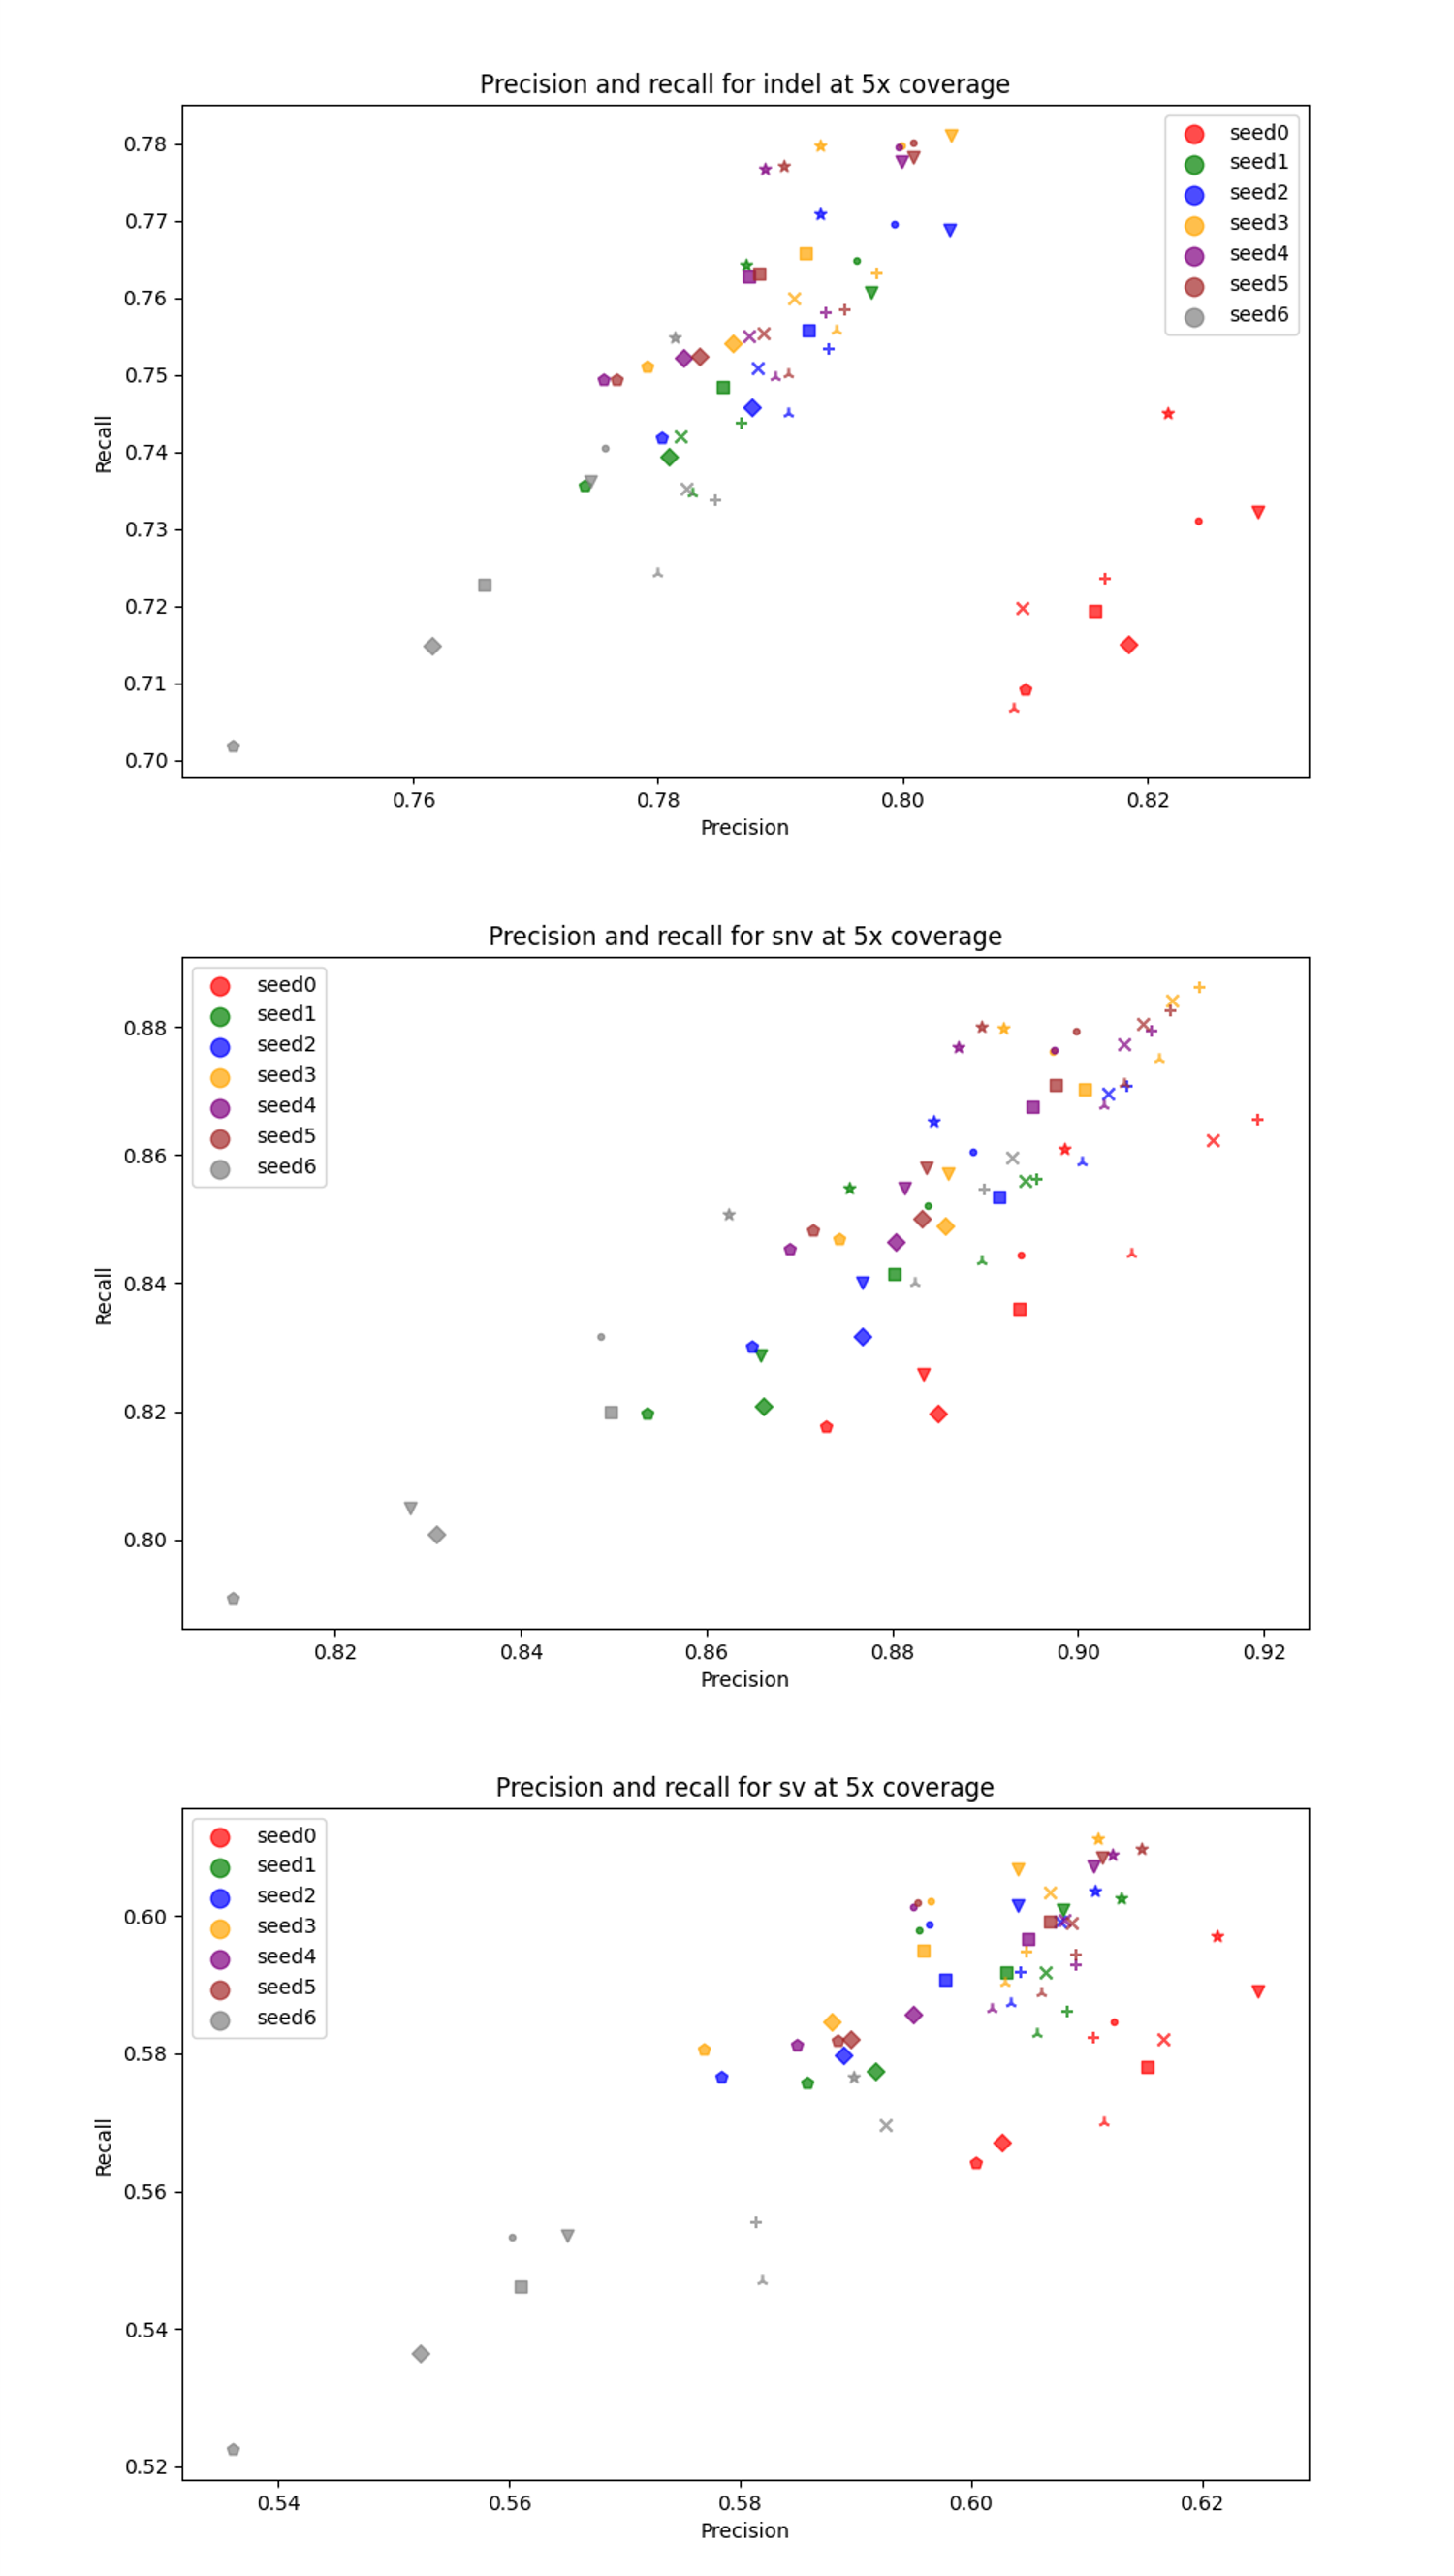
\includegraphics[scale=0.5]{figures/Sensitivity_genotyping_5x.png}
	\caption{Scatter plots for precision and recall of genotyping for \textbf{5-fold coverage} under \textbf{sensitivity case}. The results are calculated for each sample with each seed, and each sample is denoted by a unique symbol on the plots.}
	\label{fig:sensitivity_genotyping_5x} % \ref{this label}
\end{figure}
\begin{figure}[ht!]
	\centering
	\includegraphics[scale=0.5]{figures/Sensitivity_genotping_30x.png}
	\caption{Scatter plots for precision and recall of genotyping for \textbf{30-fold coverage} under \textbf{sensitivity case}. The results are calculated for each sample with each seed, and each sample is denoted by a unique symbol on the plots.}
	\label{fig:sensitivity_genotyping_30x} % \ref{this label}
\end{figure}


\begin{table*}[ht!]
\begin{tabular*}{\textwidth}{@{\extracolsep{\fill}}llllll@{\extracolsep{\fill}}}
\toprule
   &         &               wGC &         Precision &            Recall &           F-score \\
Variant & Seed &                   &                   &                   &                   \\
\midrule
indel & seed0  & 0.830(SE=0.010)&  0.799(SE=0.009)&  0.781(SE=0.013)&  0.790(SE=0.011) \\
   & seed1 & 0.823(SE=0.008)&  0.791(SE=0.008)&  0.763(SE=0.013)&  0.776(SE=0.010)\\
   & seed2 & 0.811(SE=0.009)&  0.780(SE=0.010)&  0.745(SE=0.013) & 0.762(SE=0.011)\\
   & seed3 & 0.800(SE=0.012)&0.772(SE=0.013)& 0.729(SE=0.015)& 0.750(SE=0.013)\\
\midrule
snv & seed0  & 0.906(SE=0.005)&  0.909(SE=0.006)&  0.881(SE=0.008)&  0.894(SE=0.006) \\
   & seed1 &0.904(SE=0.010)&  0.894(SE=0.013)&  0.869(SE=0.013)&  0.881(SE=0.013)\\
   & seed2 & 0.889(SE=0.015)&  0.871(SE=0.022)&  0.846(SE=0.019) & 0.858(SE=0.020)\\
   & seed3 & 0.877(SE=0.021)& 0.855(SE=0.030)& 0.828(SE=0.025)& 0.841(SE=0.027)\\
\midrule
sv & seed0  & 0.704(SE=0.010)&  0.632(SE=0.008)&  0.638(SE=0.010) & 0.635(SE=0.009) \\
   & seed1 & 0.676(SE=0.009)&  0.603(SE=0.010)&  0.596(SE=0.010)&  0.600(SE=0.009)\\
   & seed2 & 0.657(SE=0.010)&  0.586(SE=0.013)&  0.570(SE=0.012)&  0.578(SE=0.012)\\
   & seed3 & 0.641(SE=0.013)& 0.569(SE=0.019)& 0.551(SE=0.016)& 0.560(SE=0.017)\\
\bottomrule
\end{tabular*}
\caption{Genotyping results for \textbf{5-fold coverage} under \textbf{care position} \label{table:care-5x}}
\end{table*}
\begin{table*}[ht!]
\begin{tabular*}{\textwidth}{@{\extracolsep{\fill}}llllll@{\extracolsep{\fill}}}
\toprule
   &         &               wGC &         Precision &            Recall &           F-score \\
Variant & Seed &                   &                   &                   &                   \\
\midrule
indel & seed0  & 0.884(SE=0.017)&0.874(SE=0.012)&  0.853(SE=0.024)&  0.863(SE=0.018) \\
   & seed1 &0.888(SE=0.019)&  0.881(SE=0.013)&  0.846(SE=0.030)&  0.863(SE=0.022)\\
   & seed2 & 0.884(SE=0.019)&  0.879(SE=0.013)&  0.839(SE=0.032)&  0.858(SE=0.022)\\
   & seed3 & 0.884(SE=0.019)&  0.885(SE=0.012)&  0.836(SE=0.032) & 0.859(SE=0.022)\\
   
\midrule
snv & seed0 & 0.957(SE=0.003)&  0.974(SE=0.003)&  0.952(SE=0.005)&  0.963(SE=0.004)\\
   & seed1 & 0.970(SE=0.003)&  0.976(SE=0.003)&  0.963(SE=0.005)&  0.969(SE=0.004)\\
   & seed2 & 0.970(SE=0.003)&  0.974(SE=0.003)&  0.963(SE=0.005)&  0.968(SE=0.004)\\
   & seed3 & 0.972(SE=0.002) &0.978(SE=0.002)&0.964(SE=0.004)& 0.971(SE=0.002)\\
  
\midrule
sv & seed0  & 0.733(SE=0.02)&  0.675(SE=0.013)&  0.671(SE=0.019)&  0.673(SE=0.014) \\
   & seed1 & 0.717(SE=0.015)&  0.664(SE=0.011)&  0.642(SE=0.020)&  0.653(SE=0.014)\\
   & seed2 & 0.706(SE=0.015)&  0.657(SE=0.010)&  0.626(SE=0.020)&  0.641(SE=0.013)\\
   & seed3 & 0.701(SE=0.016)&0.660(SE=0.012)&0.618(SE=0.02)&0.638(SE=0.013)\\
   
\bottomrule
\end{tabular*}
\caption{Genotyping results for \textbf{30-fold coverage } under \textbf{care position}\label{table:care-30x}}
\end{table*}
\begin{figure}[ht!]
	\centering
	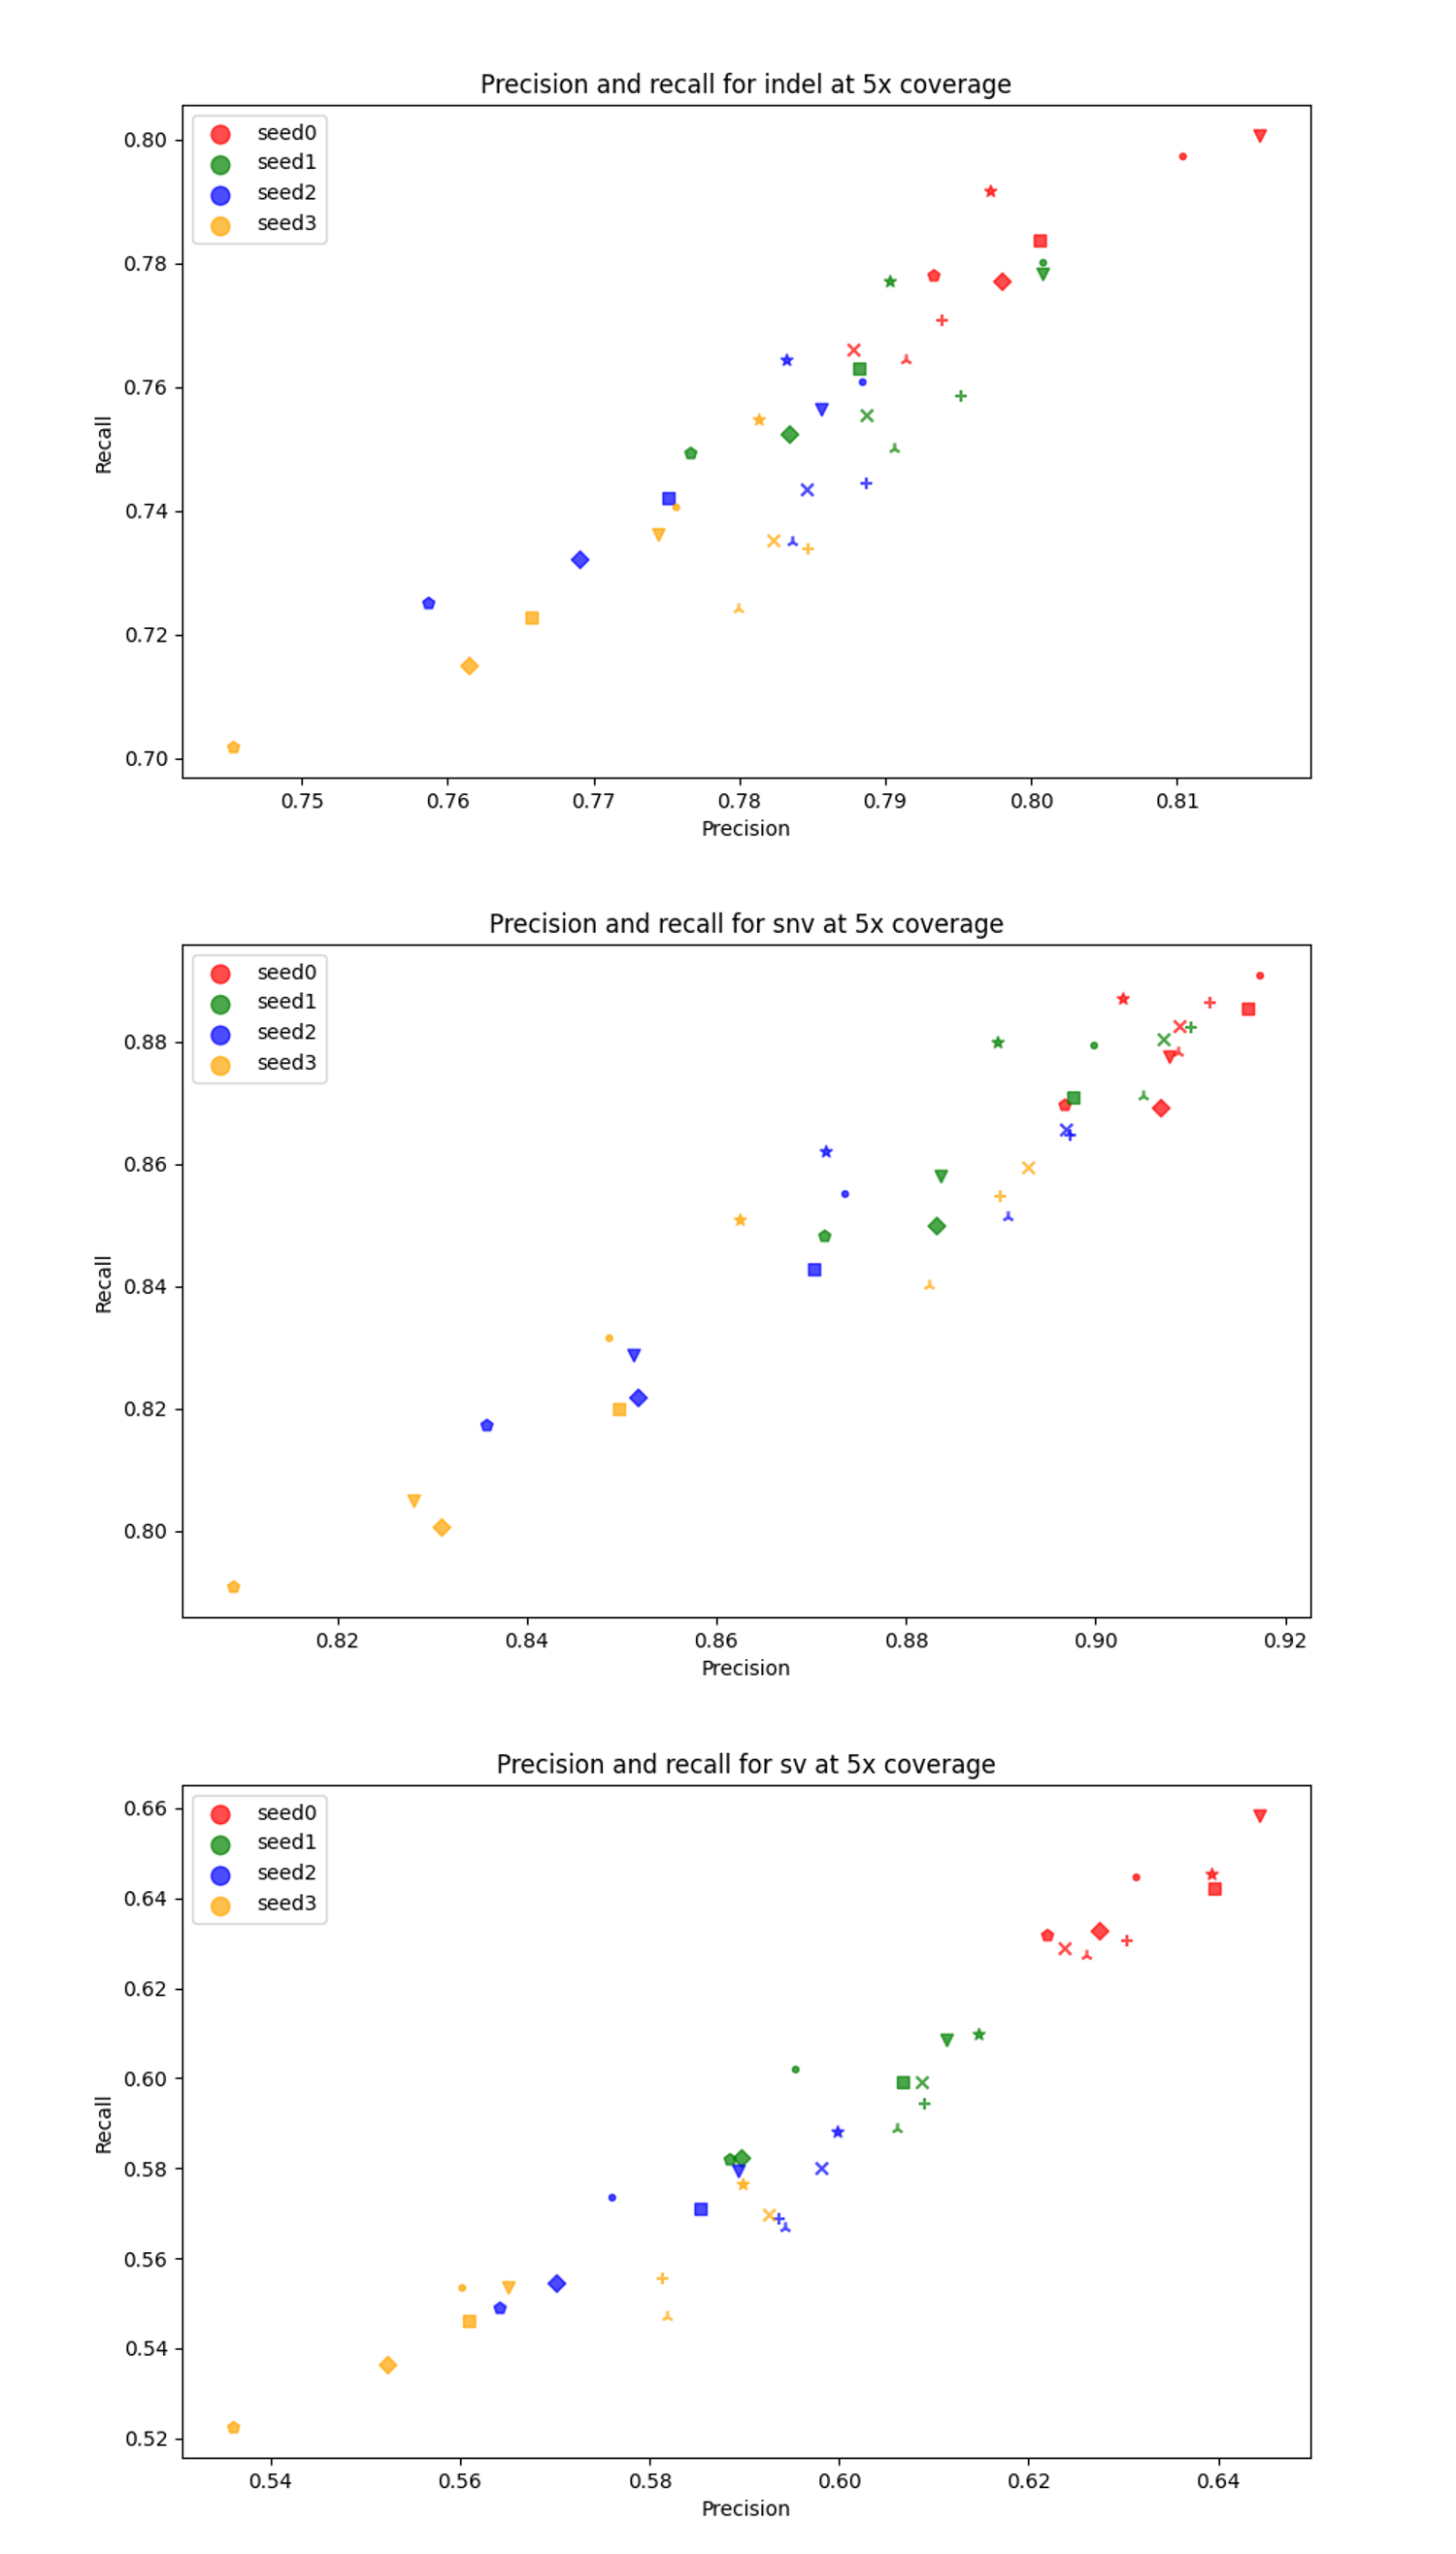
\includegraphics[scale=0.5]{figures/care_genotyping_5x.png}
	\caption{Scatter plots for precision and recall of genotyping for \textbf{5-fold coverage} under \textbf{care position case}. The results are calculated for each sample with each seed, and each sample is denoted by a unique symbol on the plots.}
	\label{fig:care_genotyping_5x} % \ref{this label}
\end{figure}
\begin{figure}[ht!]
	\centering
	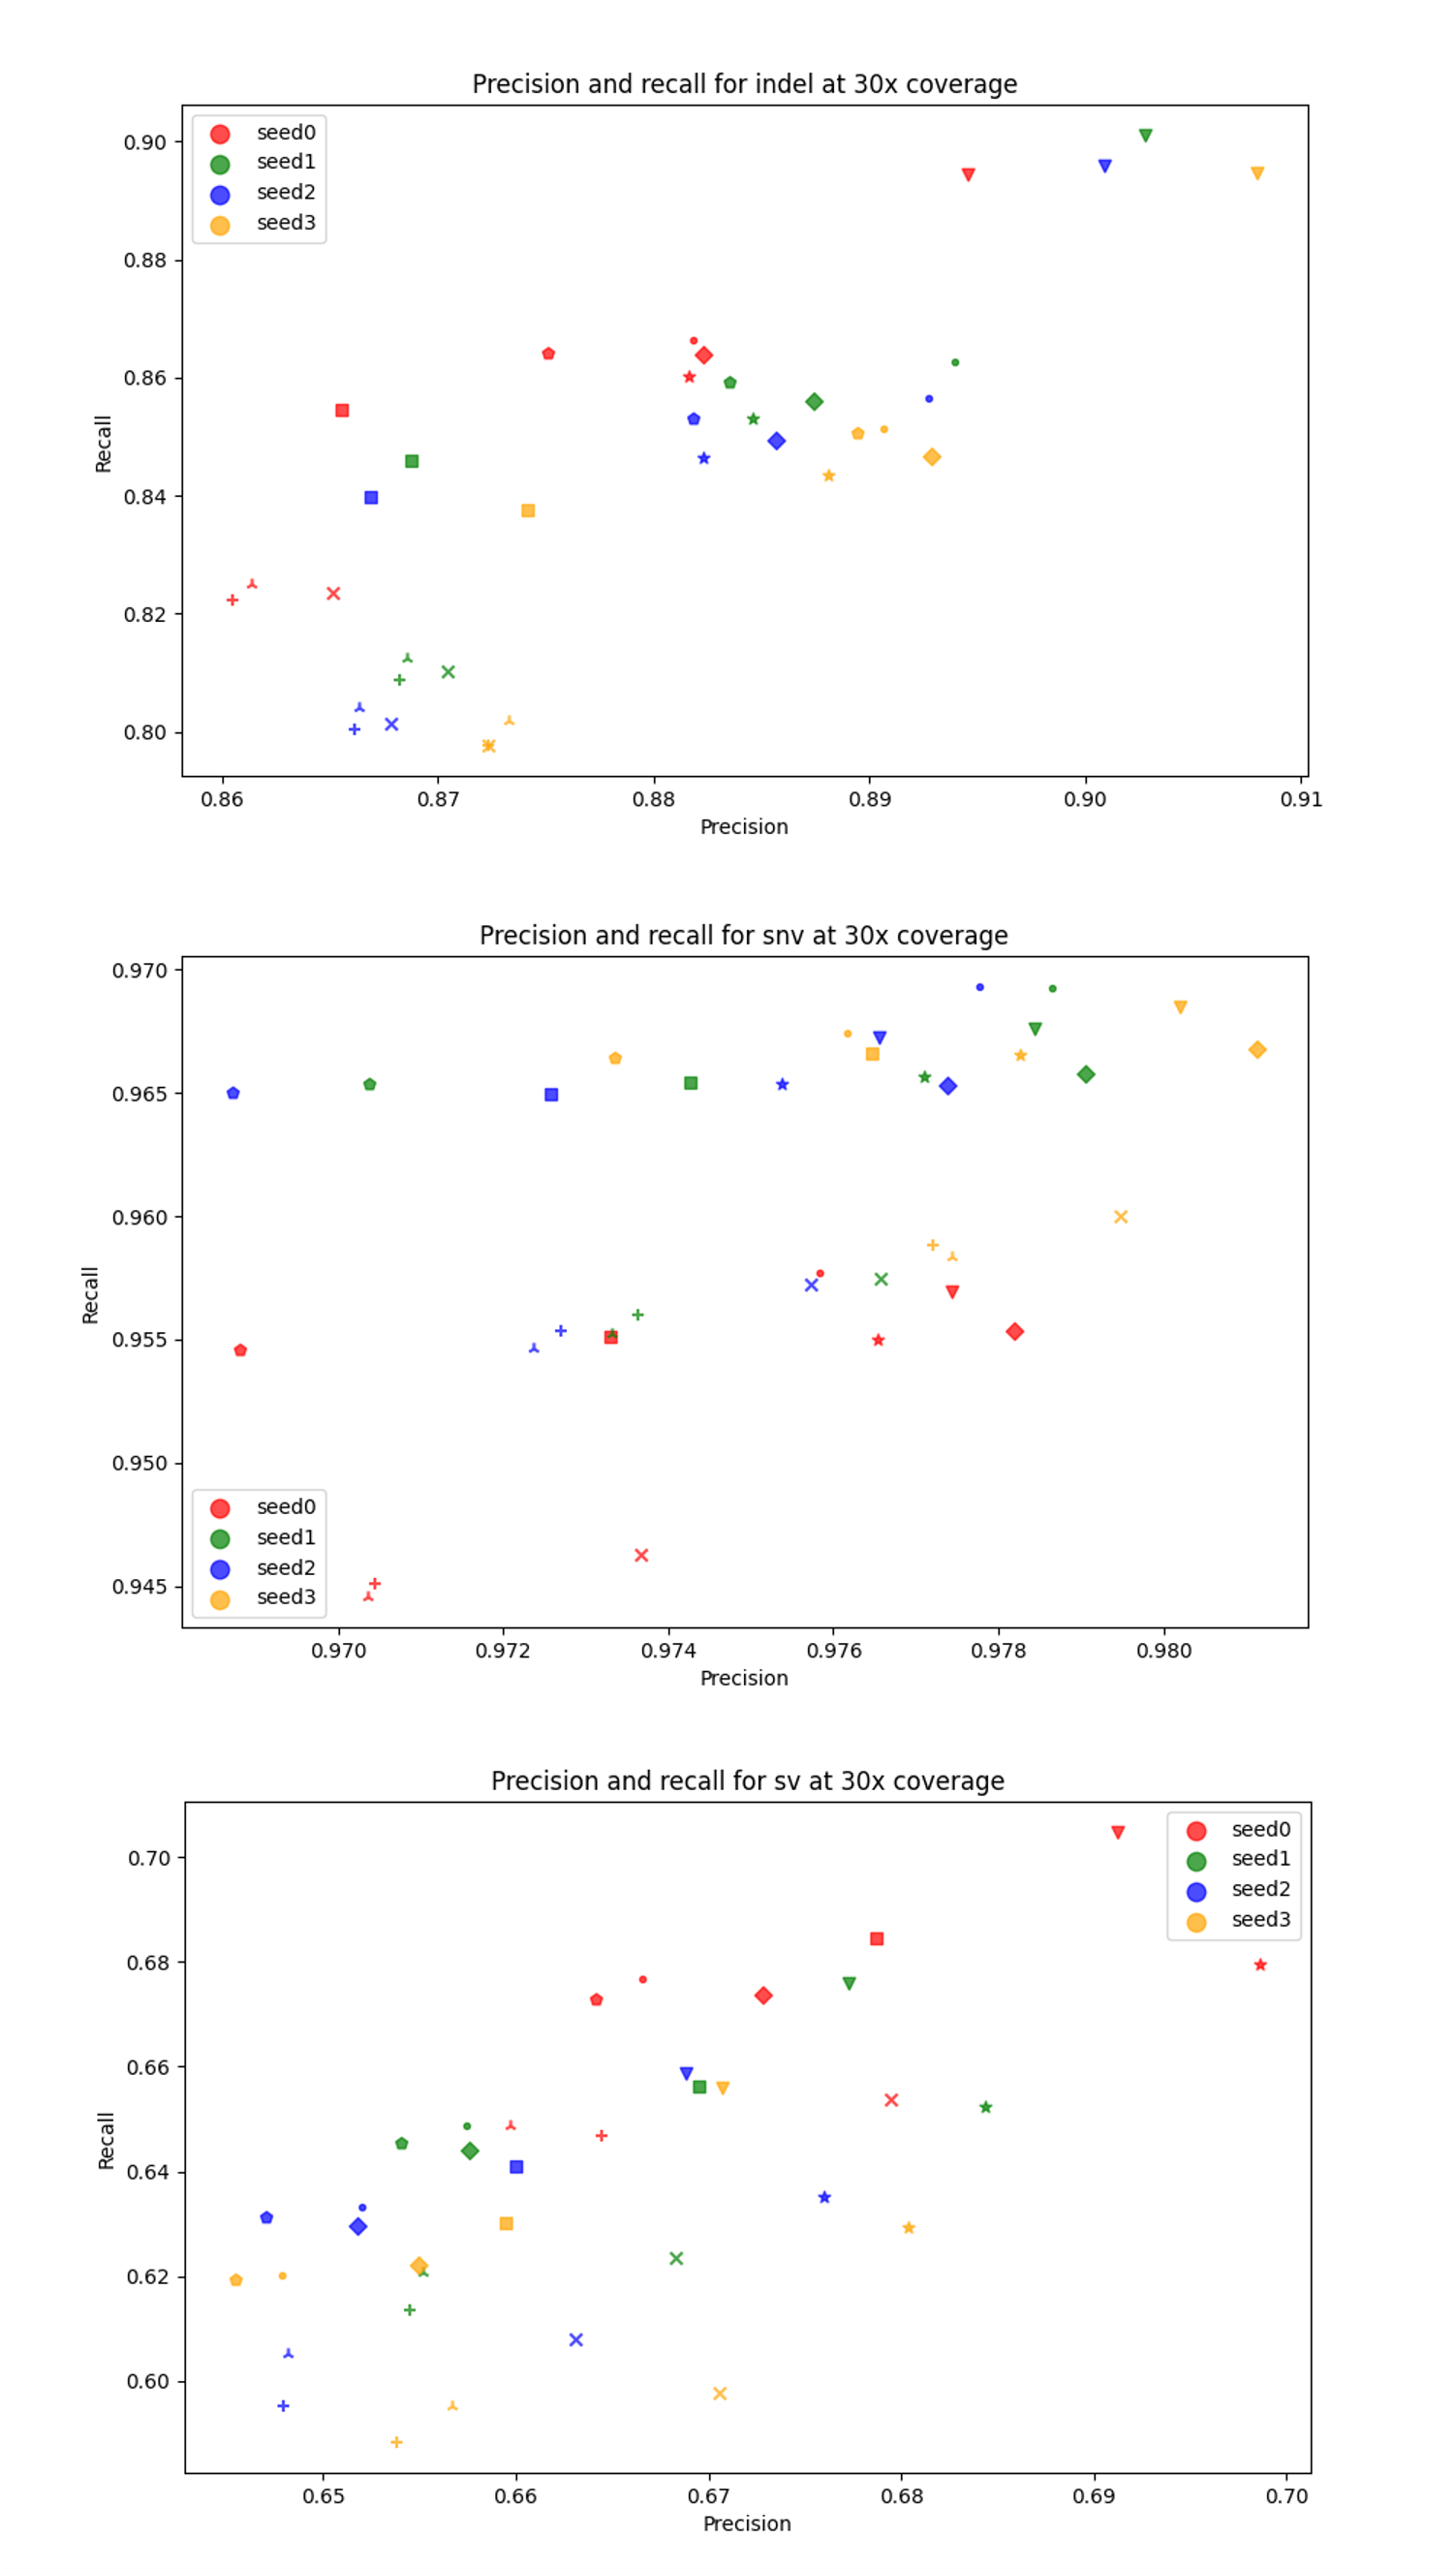
\includegraphics[scale=0.5]{figures/care_genotyping_30x.png}
	\caption{Scatter plots for precision and recall of genotyping for \textbf{30-fold coverage} under \textbf{care position case}. The results are calculated for each sample with each seed, and each sample is denoted by a unique symbol on the plots.}
	\label{fig:care_genotyping_30x} % \ref{this label}
\end{figure}

\begin{table*}[ht!]
\begin{tabular*}{\textwidth}{@{\extracolsep{\fill}}llllll@{\extracolsep{\fill}}}
\toprule
   &         &               wGC &         Precision &            Recall &           F-score \\
Variant & Seed &                   &                   &                   &                   \\
\midrule
indel & seed0  & 0.774(SE=0.009)& 0.817(SE=0.007)& 0.722(SE=0.012)& 0.767(SE=0.009) \\
   & seed1 & 0.817(SE=0.008)&  0.803(SE=0.007)&  0.761(SE=0.012)&  0.781(SE=0.009)\\
   & seed2 & 0.823(SE=0.008)& 0.790(SE=0.008)& 0.763(SE=0.012)& 0.776(SE=0.010)\\
   & seed3 &  0.816(SE=0.009)&  0.774(SE=0.012)&  0.753(SE=0.013)&  0.763(SE=0.011)\\
\midrule
snv & seed0  & 0.877(SE=0.014)& 0.896(SE=0.015)& 0.842(SE=0.018)& 0.868(SE=0.016) \\
   & seed1 &0.896(SE=0.010)&  0.896(SE=0.012)&  0.861(SE=0.013)&  0.878(SE=0.012)\\
   & seed2 & 0.904(SE=0.010)& 0.894(SE=0.013)& 0.869(SE=0.013)& 0.881(SE=0.012)\\
   & seed3 & 0.901(SE=0.013)&  0.883(SE=0.016)&  0.864(SE=0.016)&  0.873(SE=0.016)\\
\midrule
sv & seed0  & 0.650(SE=0.010)& 0.613(SE=0.008)& 0.579(SE=0.011)& 0.596(SE=0.009) \\
   & seed1 & 0.669(SE=0.009)&  0.610(SE=0.008)&  0.592(SE=0.009)&  0.601(SE=0.008)\\
   & seed2 & 0.676(SE=0.009)&0.603(SE=0.010)&0.596(SE=0.010)&0.600(SE=0.009)\\
   & seed3 & 0.676(SE=0.011)&  0.595(SE=0.014)&  0.594(SE=0.013)&  0.594(SE=0.013)\\
\bottomrule
\end{tabular*}
\caption{Genotyping results for \textbf{5-fold coverage} under \textbf{length variation} \label{table:len-5x}}
\end{table*}
\begin{table*}[ht!]
\begin{tabular*}{\textwidth}{@{\extracolsep{\fill}}llllll@{\extracolsep{\fill}}}
\toprule
   &         &               wGC &         Precision &            Recall &           F-score \\
Variant & Seed &                   &                   &                   &                   \\
\midrule
indel & seed0  & 0.825(SE=0.015)&  0.889(SE=0.012)&  0.790(SE=0.022)&  0.836(SE=0.017) \\
   & seed1 &0.876(SE=0.018)&  0.882(SE=0.012)&  0.838(SE=0.027)&  0.859(SE=0.020)\\
   & seed2 & 0.888(SE=0.019)& 0.881(SE=0.013)& 0.846(SE=0.030)& 0.863(SE=0.022)\\
   & seed3 & 0.890(SE=0.019)&  0.878(SE=0.013)&  0.846(SE=0.032)&  0.862(SE=0.022)\\
   
\midrule
snv & seed0 & 0.942(SE=0.002)& 0.977(SE=0.003)& 0.937(SE=0.003)& 0.957(SE=0.002)\\
   & seed1 & 0.962(SE=0.002)&  0.977(SE=0.003)&  0.956(SE=0.004)&  0.966(SE=0.003)\\
   & seed2 & 0.970(SE=0.003)& 0.976(SE=0.003)& 0.963(SE=0.005)& 0.969(SE=0.004)\\
   & seed3 & 0.972(SE=0.004)&  0.973(SE=0.003)&  0.965(SE=0.006)&  0.969(SE=0.004)\\
  
\midrule
sv & seed0  & 0.682(SE=0.013)& 0.671(SE=0.011)& 0.616(SE=0.015) & 0.642(SE=0.011) \\
   & seed1 & 0.705(SE=0.015)&  0.664(SE=0.012)&  0.633(SE=0.018)&  0.648(SE=0.013)\\
   & seed2 & 0.717(SE=0.015)& 0.664(SE=0.011)& 0.642(SE=0.020)& 0.653(SE=0.014)\\
   & seed3 & 0.724(SE=0.016)&  0.664(SE=0.011)&  0.648(SE=0.021)&  0.656(SE=0.015)\\
   
\bottomrule
\end{tabular*}
\caption{Genotyping results for \textbf{30-fold coverage } under \textbf{length variation}\label{table:len-30x}}
\end{table*}

\begin{figure}[ht!]
	\centering
	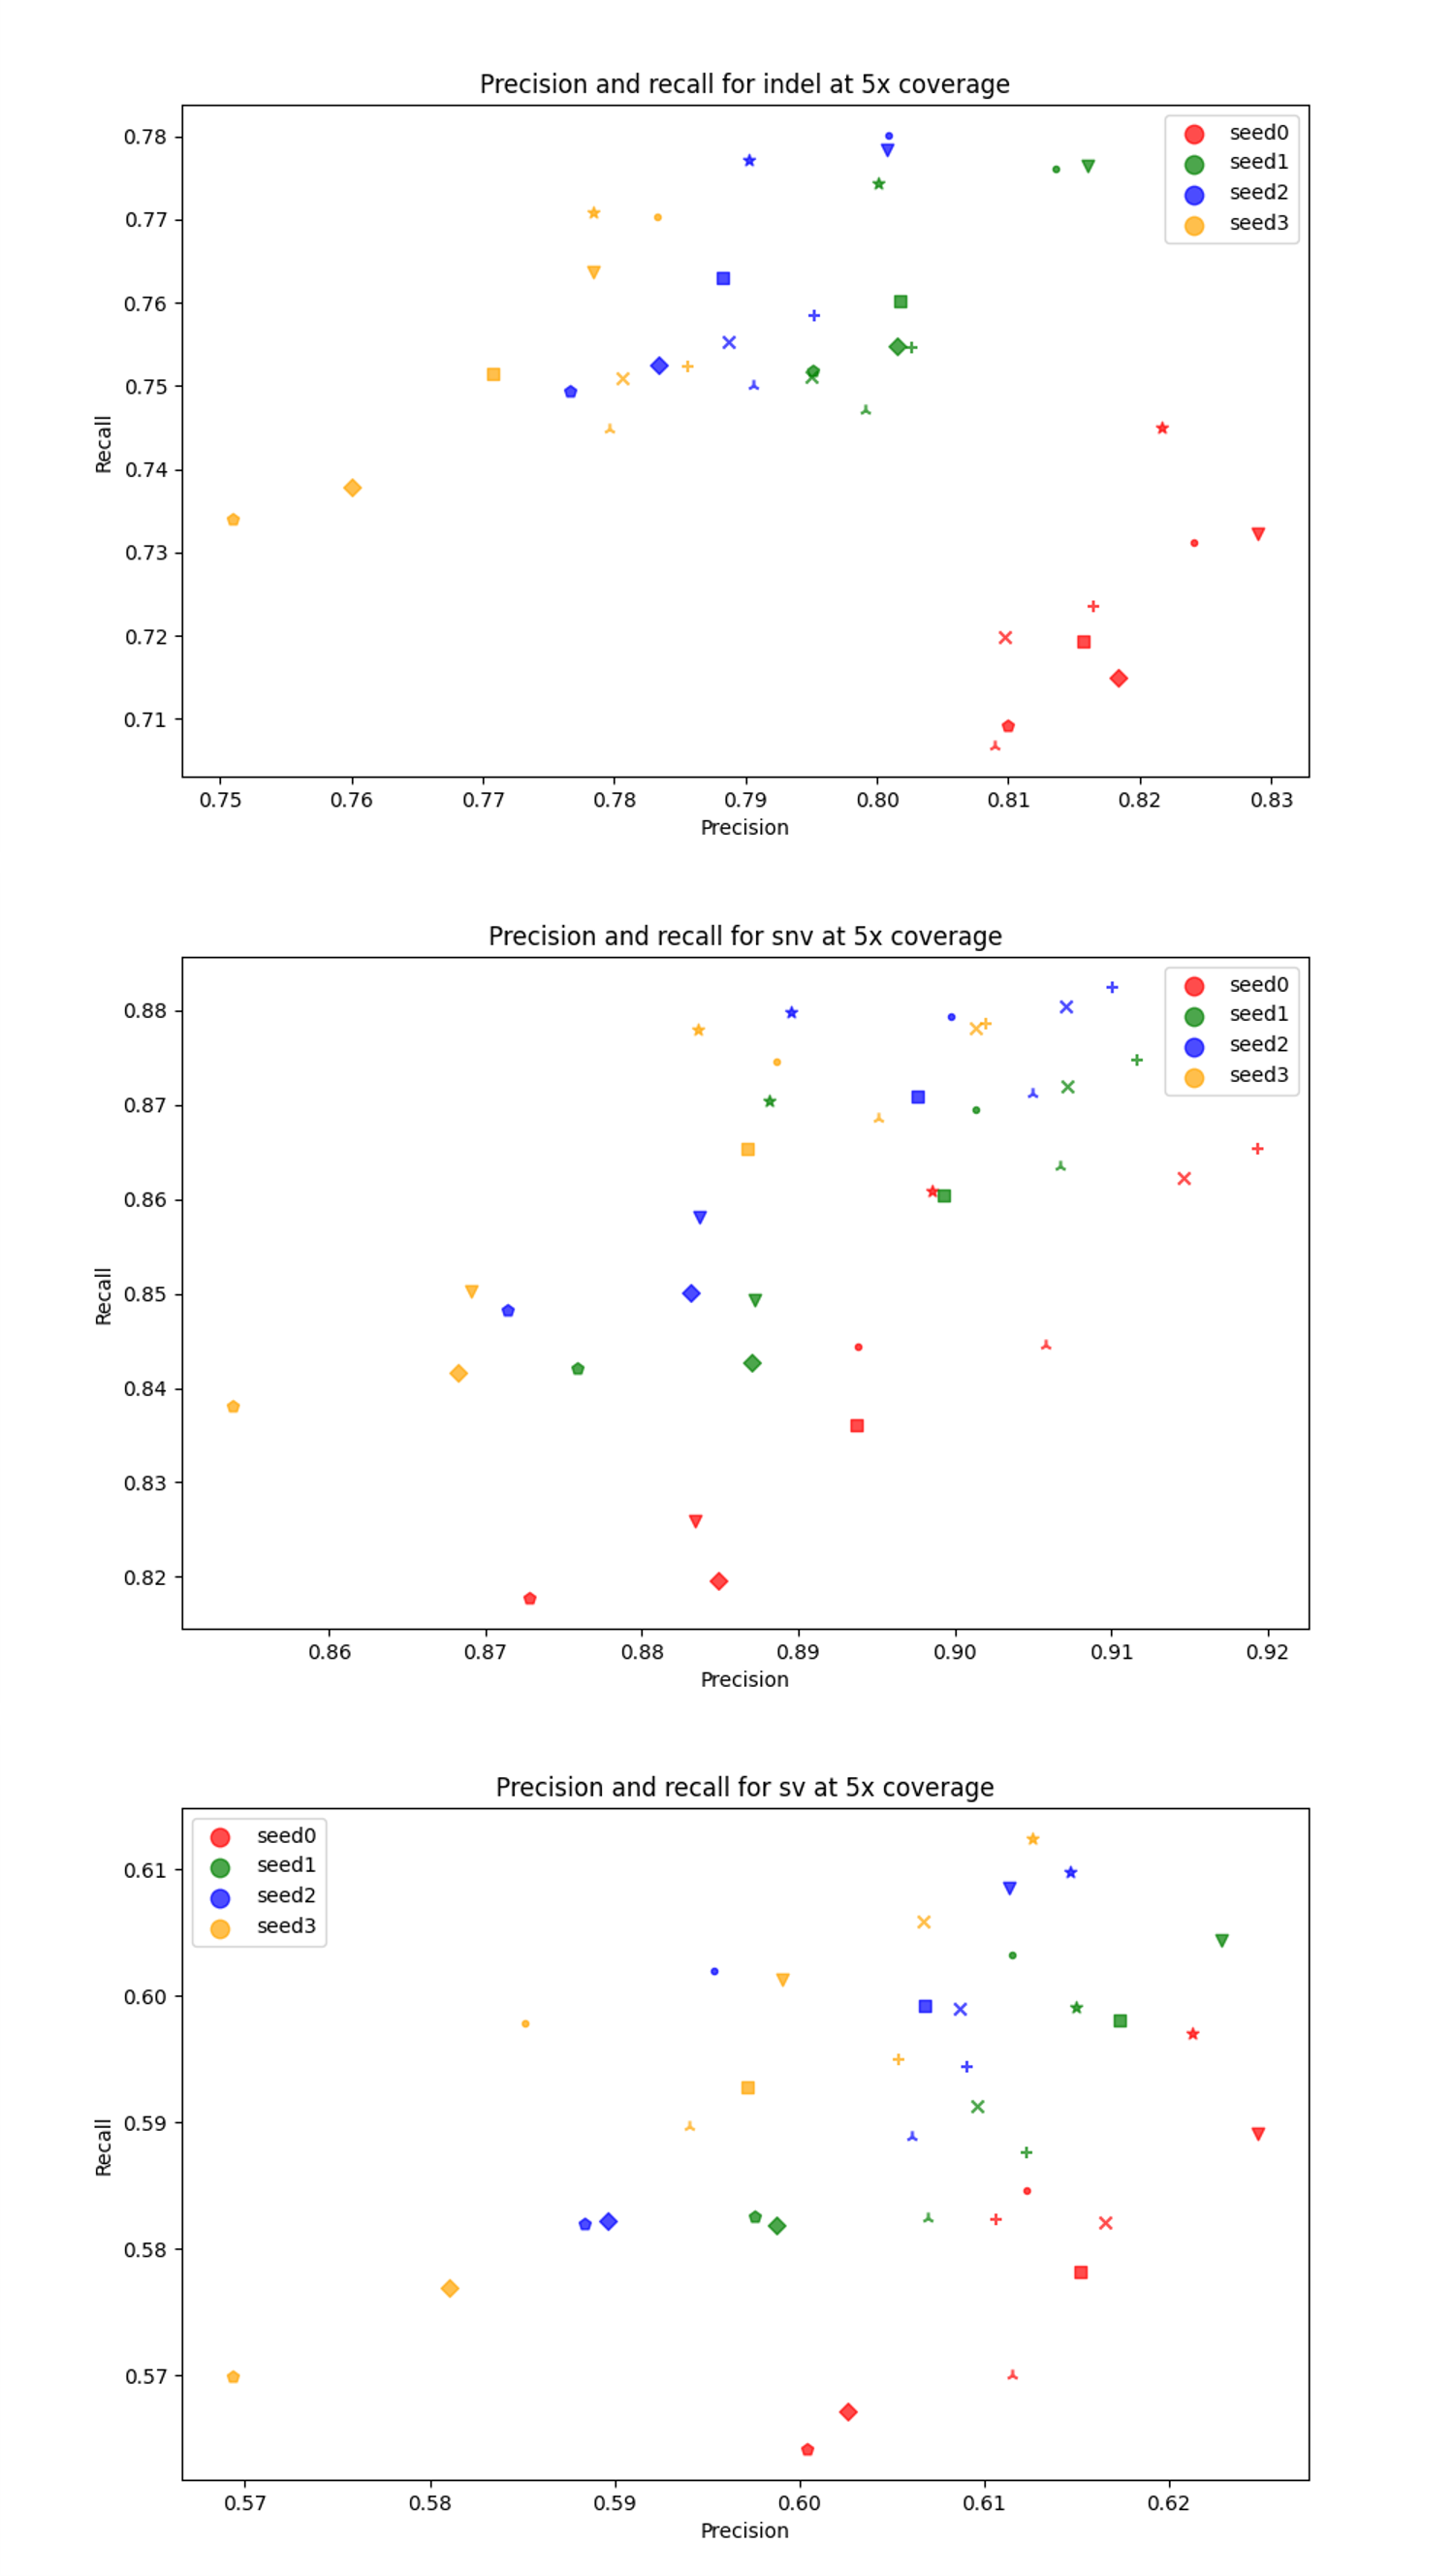
\includegraphics[scale=0.5]{figures/len_genotyping_5x.png}
	\caption{Scatter plots for precision and recall of genotyping for \textbf{5-fold coverage} under \textbf{length variation case}. The results are calculated for each sample with each seed, and each sample is denoted by a unique symbol on the plots.}
	\label{fig:len_genotyping_5x} % \ref{this label}
\end{figure}
\begin{figure}[ht!]
	\centering
	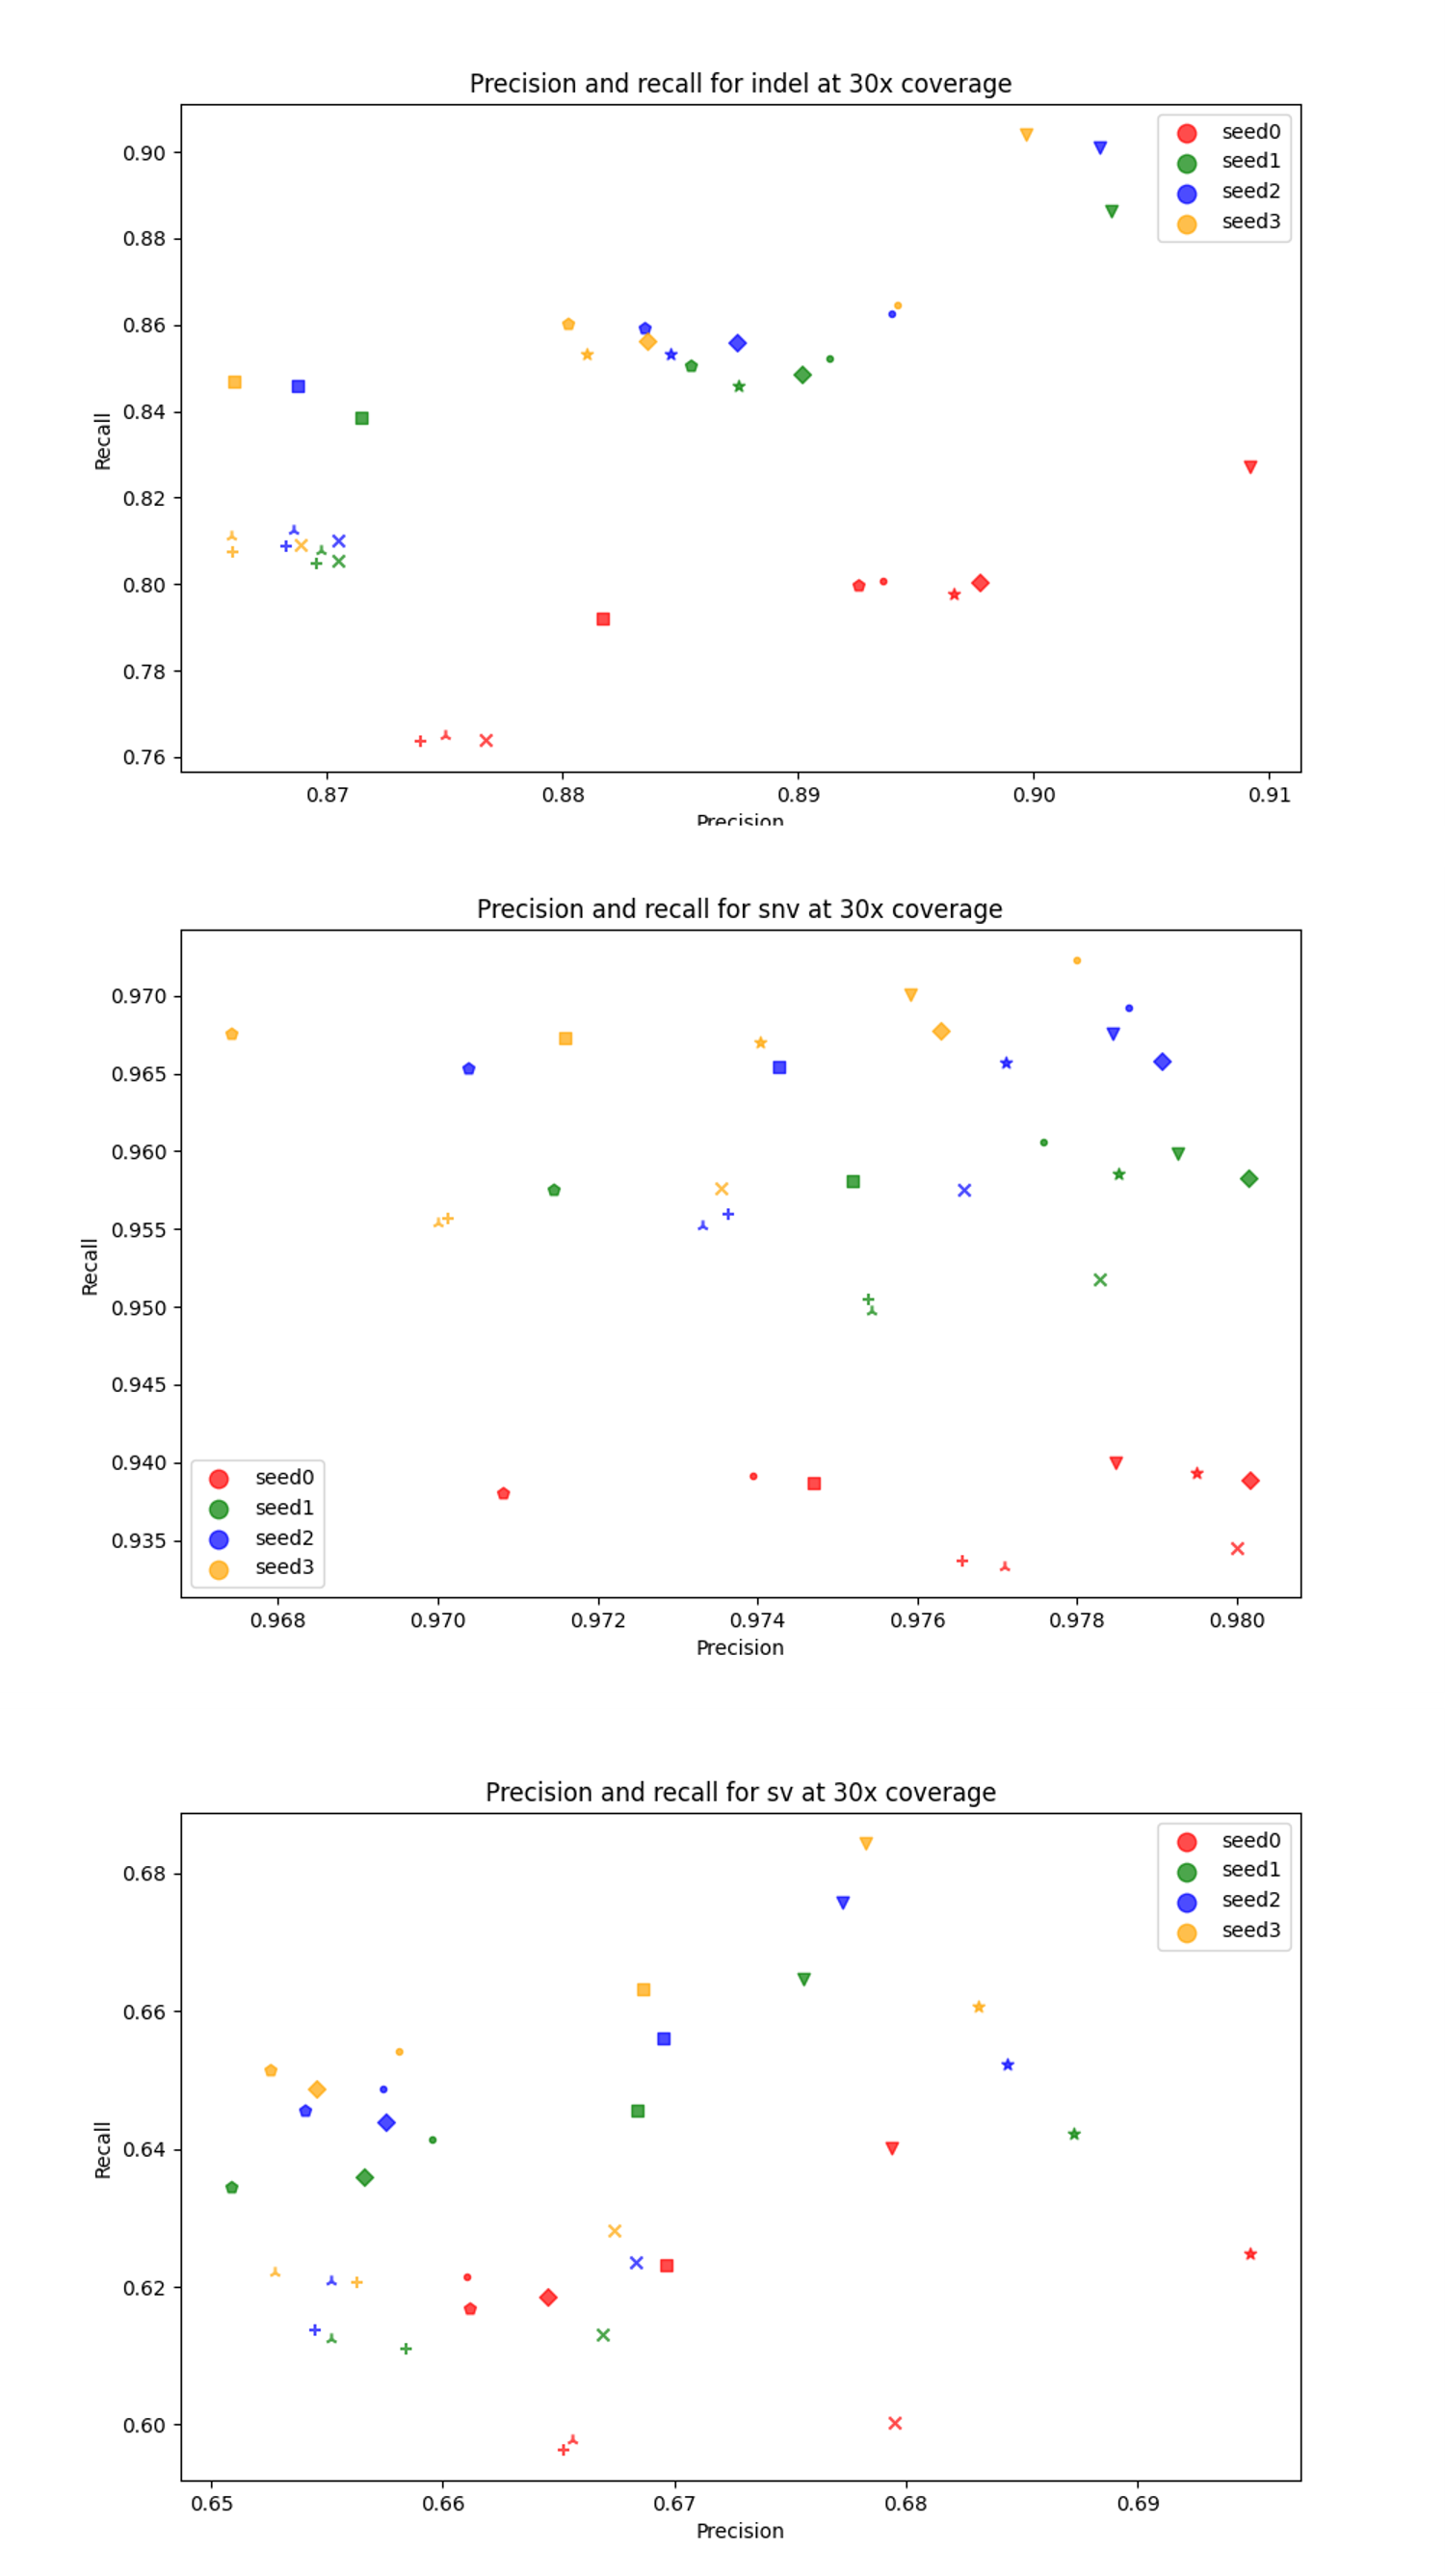
\includegraphics[scale=0.5]{figures/len_genotyping_30x.png}
	\caption{Scatter plots for precision and recall of genotyping for \textbf{30-fold coverage} under \textbf{length variation case}. The results are calculated for each sample with each seed, and each sample is denoted by a unique symbol on the plots.}
	\label{fig:len_genotyping_30x} % \ref{this label}
\end{figure}

\chapter{Discussion \& Future Works}
MaskedPanGenie is an alignment-free genotyping tool that utilizes spaced k-mers. However, its main drawback is the high runtime, which means that obtaining relatively better genotyping results comes at a significant time cost. In our study, generating results for a single spaced seed in nine samples alone took nearly a week. In contrast, the new version of MaskedPanGenie is capable of producing genotyping results for 2-3 spaced seeds in the same timeframe(Table \ref{table:RuntimeSpaced}). Nevertheless, there is still room for optimization in terms of runtime.

\begin{table}[h!]
	\centering
	\begin{tabular*}{\textwidth}{@{\extracolsep{\fill}}cccc@{\extracolsep{\fill}}}
        \toprule
        Method & Coverage & Mean & Whole Runtime\\
        \midrule
        MaskedPanGenie(i)& 5x & 4h:28min & 1d:16h:14min\\
        MaskedPanGenie(ii)& 5x & 2h:18min & 20h:39min\\
        \midrule
        MaskedPanGenie(i)& 30x & 9h:11min & 3d:10h:43min\\
        MaskedPanGenie(ii)& 30x & 3h:47min & 1d:3h:47min\\
        \bottomrule 
	\end{tabular*}
	\caption{The average time and total time required to generate a single spaced seed in nine samples across different coverage compared between Häntze's MaskedPanGenie(i) and the revised MaskedPanGenie(ii).}
	\label{table:RuntimeSpaced}
\end{table}

In the new version of MaskedPanGenie, two aspects can be further optimized. Firstly, counting k-mers in reads and the pangenome graph can be optimized by exploring accelerated algorithms such as spaced k-mer seed hashing, as mentioned in the Method chapter. I attempted one such algorithm, FSH, but the potential time cost did not yield the expected results. Therefore, alternative algorithms could be explored and implemented.

Secondly, MaskedPanGenie employs a relatively simple approach of using a provided spaced seed to mask all k-mers of a variant bubble and comparing the counts of spaced k-mers instead. This approach, though straightforward, requires more time due to the querying of k-mer occurrences. Thus, optimizing this step could lead to improved genotyping results within a better timeframe.

By further optimizing these two steps, MaskedPanGenie can achieve superior genotype results compared to PanGenie, while maintaining a reasonable runtime.

In addition to studying the factors affecting genotyping results based on spaced seed patterns, we investigated the impact of three factors: (1) the level of sensitivity, (2) the number of care positions, and (3) variations in seed length. Our current analysis suggests that selecting a spaced seed with higher sensitivity, fewer care positions, and longer length tends to yield better genotyping results. However, not all data consistently demonstrate this trend, and inconsistencies exist between genotyping results obtained from low-coverage and high-coverage reads. Consequently, we currently lack a definitive explanation for these observations. Nonetheless, there are two directions we can explore further.

Firstly, we can consider using different datasets or increasing the amount of data. In this study, we used the dataset provided by the original authors, which may have fewer variant information compared to the dataset used by PanGenie's authors to construct the pangenome graph. Analyzing the genotyping results under these changes, incorporating a dataset containing known variations, may provide additional insights and deeper explanations.

Secondly, we can explore alternative spaced seed patterns~\cite{Noe2017SeedSelection}, such as indel seeds, neighbor seeds, subset seeds, or other possibly related spaced seed patterns. Additionally, investigating different algorithms for generating more suitable spaced seeds could be beneficial. Generating an optimal spaced seed is known to be a challenging problem, encompassing sensitivity computation and seed design.

\chapter{Conclusion}
In this study, we proposed an improved modification to the MaskedPanGenie pipeline, which utilizes spaced seed for alignment-free k-mer-based genotyping. Our modifications not only significantly reduce the overall execution time but also help save additional memory space. Furthermore, we have made the entire pipeline more user-friendly and accessible.

Regarding the spaced seed aspect, we have also presented an appropriate method for generating better spaced seeds. We have provided options for selecting spaced seed pattern designs and conducted related analyses on their impact on genotyping results. Although our research results in this area have not provided a definitive explanation, they can serve as a valuable reference for future studies.
\newpage
\AddToContents{Bibliography}
\printbibliography


\end{document}
